\documentclass{report}
\usepackage{hyperref}
\usepackage[ngerman]{babel}
\usepackage{amsmath}
\usepackage{amsfonts}
\usepackage{amsthm}
\usepackage{tcolorbox}
\usepackage[a4paper, total={7in, 9in}]{geometry}
\usepackage[font={scriptsize,it}]{caption}
\usepackage{scrextend}
\usepackage{graphicx}
\usepackage{caption}
\usepackage{subcaption}
\usepackage[utf8]{inputenc}
\usepackage[T1]{fontenc}
\DeclareUnicodeCharacter{2212}{-}
\usepackage{verbatim}
\usepackage{tikz}

\tikzset{
  treenode/.style = {shape=rectangle, rounded corners,
                     draw, align=center,
                     top color=white, bottom color=blue!20},
  root/.style     = {treenode, font=\Large, bottom color=red!30},
  env/.style      = {treenode, font=\ttfamily\normalsize},
  dummy/.style    = {circle,draw}
}

\tikzstyle{level 1}=[level distance=3.5cm, sibling distance=3.5cm]
\tikzstyle{level 2}=[level distance=3.5cm, sibling distance=2cm]

% floating figure for column
\newenvironment{Figure}
	{\par\medskip\noindent\minipage{\linewidth}}
	{\endminipage\par\medskip}

\theoremstyle{definition}
\newtheorem{definition}{Definition}

\theoremstyle{example}
\newtheorem*{example}{Example}

\begin{document}

\begin{titlepage}
   \vspace*{\stretch{1.0}}
   \begin{center}
      \Large\textbf{MQMO - FS20}\\
      \large\textit{Pascal Brunner - brunnpa7}
   \end{center}
   \vspace*{\stretch{2.0}}
\end{titlepage}

\tableofcontents
\newpage

\chapter{Einführung in das Operations Management}

\section{Operations Management in der Unternehmung}
Definition:\\
Operations Management beinhaltet die \textbf{Gestaltung} ('Design'), den \textbf{Betrieb} ('Operation' d.h. Planen und Steuern) und die \textbf{Optimierung} ('Improvement') aller \textbf{Systeme und Prozesse}, 
welche beteiligt sind an der \textbf{Kreation und Bereitstellung} der \textbf{Produkte und Dienstleistungen} eines Unternehmens 
\begin{itemize}
   \item OM beschäfitgt sich damit, wie ein Unternehmen \textbf{Produkte und Dienstleistungen} \textit{kreieren bzw. bereitstellen}
	\item Operations Management befasst sich mit dem Prozess von einem Delivery, Input, Process und Output. Damit wird aus dem einem Demand einen Goods oder Services erstellt. Entsprechend ist es ein zwei gleisiges Verfahren. 
	\item OM beschäfigt sich damit, Aktivitäten des Kerngeschäfts möglichst effizient darzustellen.
	\item Operations bezeichnet das Kerngeschäft des Unternehmens $\rightarrow$ Alle Systeme und Prozesse, welche die Produkte und DL des UNternehmens kreieren und bereitstellen, d.h. direkt und in wesentlichem Mass an der Wertschöpfung beteiligt sind.
	\item 
\end{itemize}
\begin{Figure}
\centering
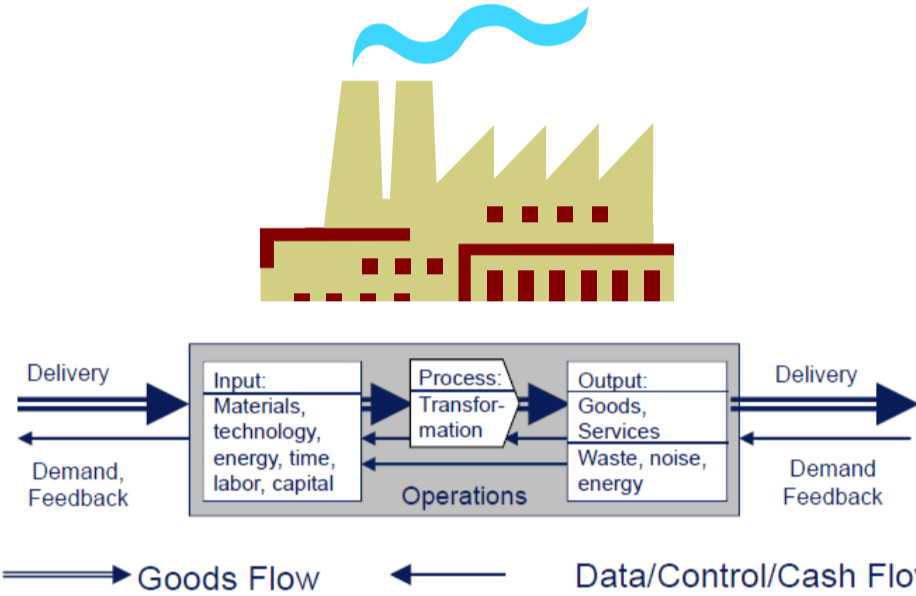
\includegraphics[width=150px]{img/OM.png}
	\captionof{figure}{OM Model}
	\label{fig:OM Model}
\end{Figure}

   \subsection{Eingliederung von Operations}
Jedes Unternehmen umfasst drei (betriebliche) Hauptfunktion:
\begin{itemize}
   \item Marketing & Sales $\rightarrow$ Werbung, Akquise, Verkauf, Beratung
   \item Product/Service Development $\rightarrow$ Entwicklung, Anpassung von Produkte
   \item Operations $\rightarrow$ Herstellung der Produkte und Dienstleistungen, Bereitstellung für den Kunden
\end{itemize}
Zusatzfunktion:
\begin{itemize}
   \item Engineering / Technology
   \item Account & Finance
   \item HR
   \item IT
\end{itemize}
\begin{Figure}
\centering
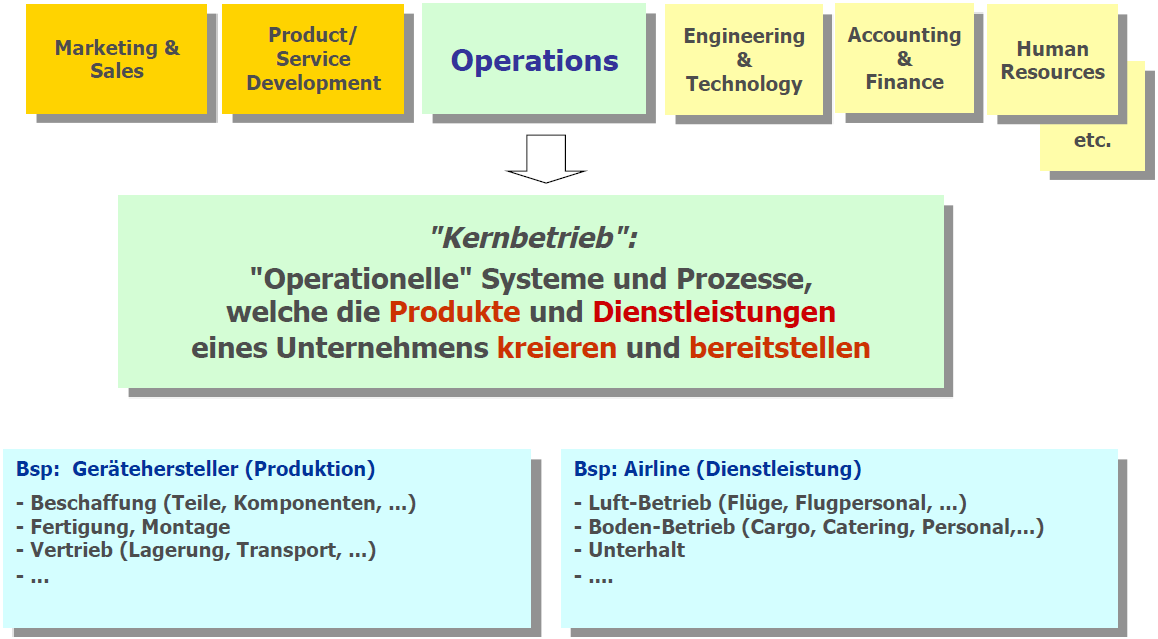
\includegraphics[width=150px]{img/Operations.png}
	\captionof{figure}{Operations zentrale betr. Funktion}
	\label{fig:Operations zentrale betr. Funktion}
\end{Figure}

      \subsubsection{Operations Management im Organigramm}
$\rightarrow$ Je nach Unternehmen, kann das Operations unterschiedlich verstreut sein, bspw.:
\begin{itemize}
   \item Fertigungsbetrieb (Produktion) $\rightarrow$ typischerweise in einem Departement zusammengefasst
   \item Airline (Dienstleistung) $\rightarrow$ Bestimmte Bereiche der Operations-Funktion in andere Departemente ausgelagert
   \item Autohersteller (Kundendienst) $\rightarrow$ Operations Funktion über vers. Departemente verteilt
\end{itemize}

   \subsection{Aufgaben des Operations Management}
\begin{Figure}
\centering
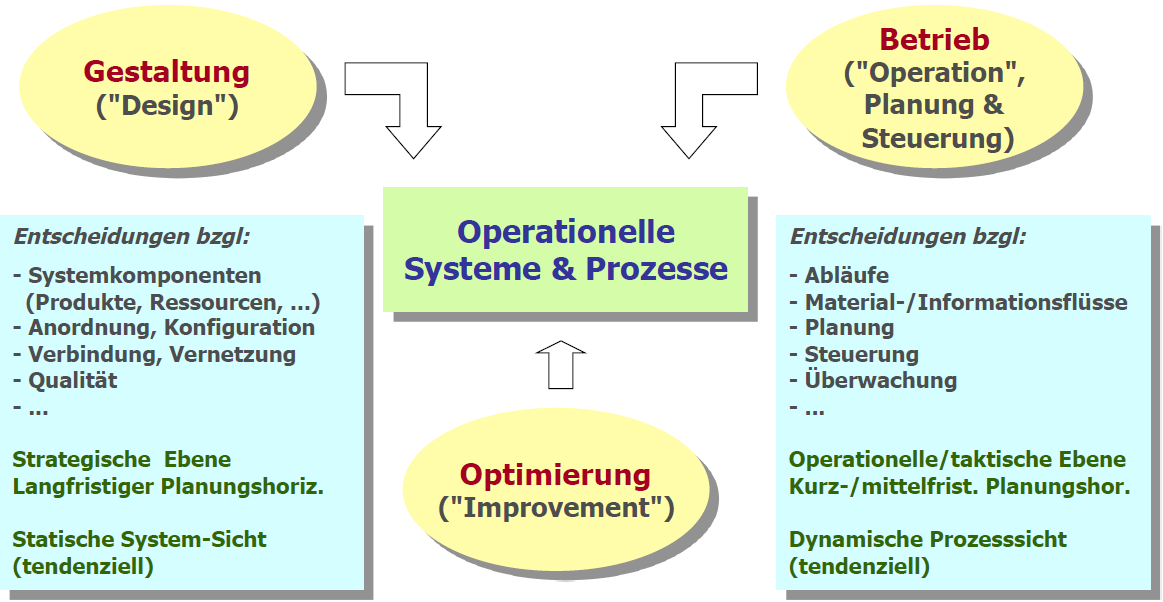
\includegraphics[width=150px]{img/OMAufgaben.png}
	\captionof{figure}{Die drei Aufgaben des OM}
	\label{fig:Die drei Aufgaben des OM}
\end{Figure}

   \subsection{Wirkungsfeld des Operations Management}
Durch die Industrie4.0 hat es eine zunehmende Ausdehnung des Wirkungsfelds
\begin{itemize}
   \item Gesamtes Leistungsspektrum: Sowohl materielle \textbf{Produkte} als auch \textbf{Dienstleistungen} $\rightarrow$ Grenze zwischen Produktions- und Dienstleistungsbetrieben zunehmend fliessend
   \item Gesamter \textbf{Lebenszyklus} des Produkts $\rightarrow$ Beschaffung - Produktion - Vertrieb \textit{Unterhalt - Entsorgung}
   \item Gesamte \textbf{Supply Chain} $\rightarrow$ Gesamtes Netzwerk von Unternehmen, welche an der Leistungserbringung beteiligt sind
\end{itemize}

%ToDo Abgrenzung zu OR und IE Kapitel 1 S. 15

   \subsection{Quantitatives Operations Management}
Definition:\\
\textbf{Analyse} und \textbf{Optimierung} von Aufgaben des OM mit Hilfe \textbf{mathematischer Modelle und Algorithmen}\\
Typisches Vorgehen:
\begin{itemize}
   \item Problem-Identifikation $\rightarrow$ kritische Teilsysteme/-prozesse identifizieren: stark ausgelastet, leistungsbestimmend, kostenintensiv, zeitkritisch
   \item Analyse $\rightarrow$ Sorgfältige Untersuchung: Das richtige Problem lösen
   \item Modellierung $\rightarrow$ Präzise Formulierung des Problems mittels mathematischer Modelle
   \item Optimierung $\rightarrow$ Berechnung guter Lösungen mit mathematischen Algorithmen
   \item Umsetzung $\rightarrow$ Übertragung / Anpassung der Resultate an das reale Problem
\end{itemize}

Decision Support: mathematische Modelle als Entscheidungshilfen (nicht 'diktatorisch')

   \subsection{Relevanz von Operations Management}
\begin{itemize}
   \item zentrale Bedeutung für Erfolg und Misserfolg eines Unternehmens
   \item 43 \% der befragten CEO's betrachtet Operations Management als \textbf{wichtigsten Know-how Bereich} für ihre Angestellten
   \item OM bildet grosser Umsatzbereich weltweit im Consulting
\end{itemize}





\section{Operations Management und Transformationsprozesse}
Operations Management beschäfigt sich im Wesentlichen mit \textbf{Transformationsprozesse}

\begin{Figure}
\centering
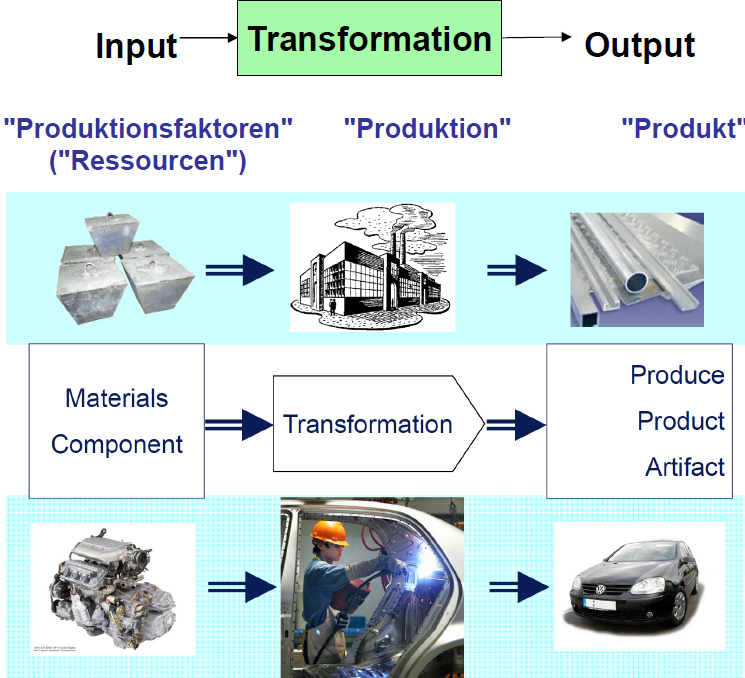
\includegraphics[width=150px]{img/OMTransformationsprozesse.png}
	\captionof{figure}{Schema des Transformationsprozess}
	\label{fig:Schema des Transformationsprozess}
\end{Figure}

   \subsection{Input}
Als Input wird der \textbf{Produktionsfaktor} bzw. die Ressourcen beschrieben
\begin{itemize}
   \item Menschliche Arbeitsleistung $\rightarrow$ objektbezogener oder dispositiver Art 
   \item Werkstoffe $\rightarrow$ Rohstoffe, Vorprodukte, Hilfsstoffe
   \item Betriebsmittel - zur aktiven Nutzung $\rightarrow$ Maschinen, Anlagen, Geräte, ...
   \item Betriebsmittel - zur passiven Nutzung $\rightarrow$ Gebäude, ...
   \item Betriebsmittel - zum Verbrauch $\rightarrow$ z.B. Energie, Kühl- und Schmiermittel, ...
   \item Information
   \item Zusatzfaktoren $\rightarrow$ z.B. Versicherungen, staatliche Leistungen, ...
   \item Kunden (bei DL)
\end{itemize}
Dazu kommen weitere Klassifikationen:
\begin{itemize}
   \item transformierende Ressourcen $\rightarrow$ Menschliche Arbeit, Betriebsmittel
   \item transformierte Ressourcen $\rightarrow$ Werkstoffe, Informationen, Kunden (bei DL)
\end{itemize}

   \subsection{Transformation}
Die Transformation ist die eigentliche \textbf{Produktion}
\begin{itemize}
   \item Physikalisch $\rightarrow$ Fertigung, Herstellung, Verbindung, ...
   \item Räumlich $\rightarrow$ Transporte, ...
   \item Zeitlich $\rightarrow$ Lagerung, ...
   \item Tausch $\rightarrow$ Handel, Detailhandel, ...
   \item Informatorisch $\rightarrow$ z.B. Telekommunikation, ...
   \item Physiologisch $\rightarrow$ z.B. Pflegedienste, ...
\end{itemize}

   \subsection{Output}
Als Output resultiert dann das \textbf{Produkt}
\begin{itemize}
   \item Materielle Produkte $\rightarrow$ Endprodukte, Zwischenprodukte, Abfallprodukte, ...
   \item Immaterielle Produkte $\rightarrow$ Dienstleistungen, Arbeitsleistungen, Information, ...
   \item Gemischte Produkte $\rightarrow$ unterschiedlichen Anteil an (Im)materielle Elemente
\end{itemize}

\section{Ziele des Operations Management}
Das Hauptziel von OM ist dass die Unternehmung eine möglichst grosse 'Leistung' $\rightarrow$ Performance erbringt.\\
Eine solche Leistung zu beschreiben und zu messen ist eine komplexe Aufgabe $\rightarrow$ \textbf{zahlreiche Leistungsmasse}.
Diese Leistungsmasse werden als KPI's (Key Performance Indicators) genannt. \\
   \subsection{Produktivität}
Ein allgemeines, grobes Leistungsmass ist die \textbf{Produktivität} $ = \frac{Output}{Input}$
Dabei ist vor allem relevant welcher \textit{Input} bzw. \textit{Output} in welchem \textit{Mass} (Geldeinheit, Zeiteinheit etc.) gemessen wird

      \subsubsection{verschiedene Produktivitätsmasse}
\textbf{Einzelfaktoren-Produktivität} Input von einzelner Ressourcen gemessen\\

\textbf{Multifaktoren-Produktivität} Input von mehreren Ressourcen gemessen (als kompatibles Mass für Input meistens Einsatzskosten in Geldeinheiten) bspw.\\
$Multifaktoren-Produktivität = \frac{Ausbringungsmenge eines Produkts}{Kosten Arbeit + Kosten Material + Kosten Energie}$

\begin{Figure}
\centering
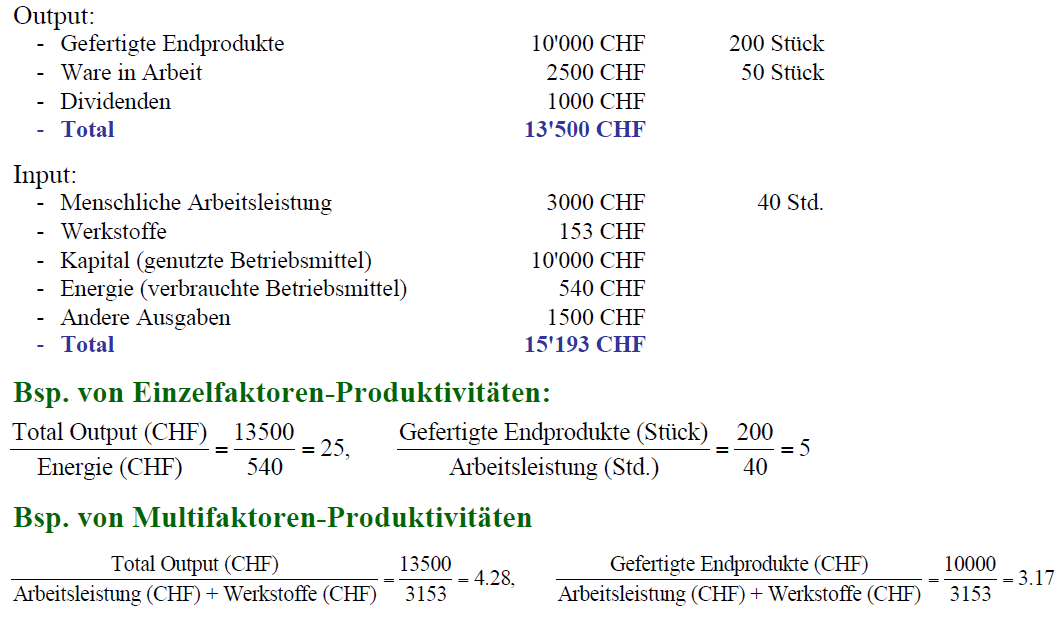
\includegraphics[width=150px]{img/ProduktivitaetNumBsp.png}
	\captionof{figure}{Numerisches Beispiel für die Produktivität}
	\label{fig:Numerisches Beispiel für die Produktivität}
\end{Figure}

      \subsubsection{Nutzen und Grenzen von Produktivitätsmasse}
\begin{itemize}
   \item relatives Mass (nicht absolut!) $\rightarrow$ aussagekräftig im Vergleich (andere Abteilungen, über Zeit, Konkurrenten)
   \item Produktivitätsmasse als operative Ziele meist ungeeignet
\end{itemize}

%ToDo Harbour Report ergänzen





\section{Entscheide des Operations Management}
\textbf{Entscheidungsbereiche (Aufgaben)}
\begin{itemize}
   \item Gestaltung ('Design')
   \item Betrieb ('Operation') $\rightarrow$ Planung (Planning) und Steuerung (Execution Control)
\end{itemize}

\begin{Figure}
\centering
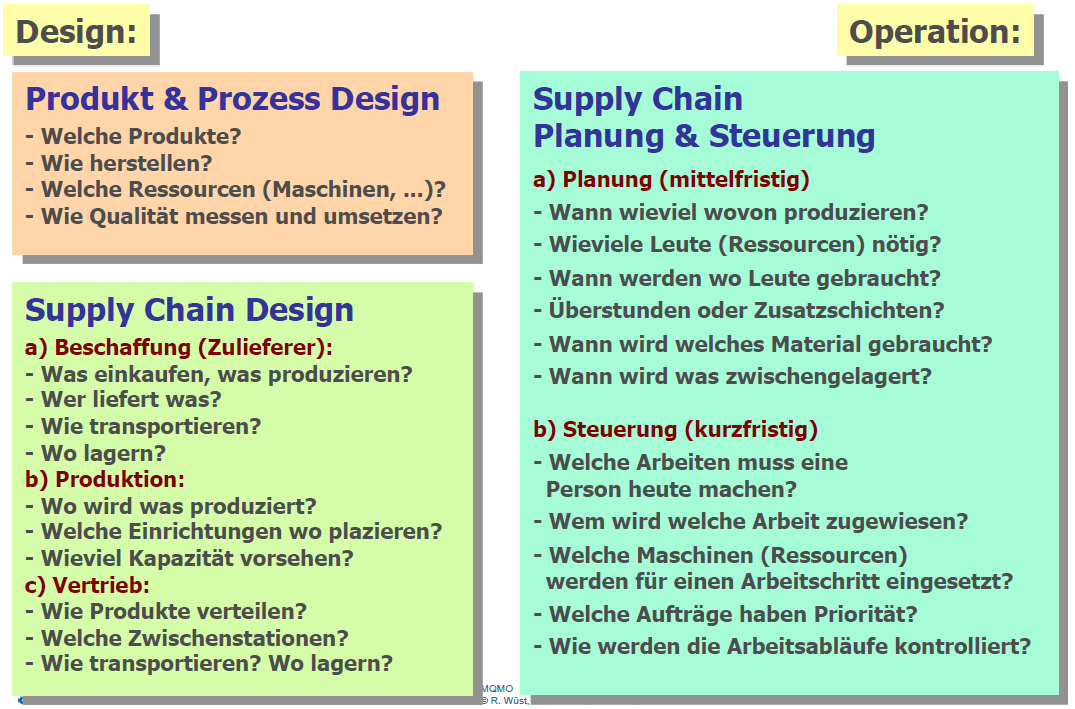
\includegraphics[width=150px]{img/OMEntscheidungsbereiche.png}
	\captionof{figure}{Entscheidungsbereiche im OM}
	\label{fig:Entscheidungsbereiche im OM}
\end{Figure}

\textbf{Entscheidungsebene (entsprechend Tragweite)}
\begin{itemize}
   \item strategisch $\rightarrow$ langfristig
   \item taktisch $\rightarrow$ mittelfristig
   \item operativ $\rightarrow$ kurzfristig
\end{itemize}

\begin{Figure}
\centering
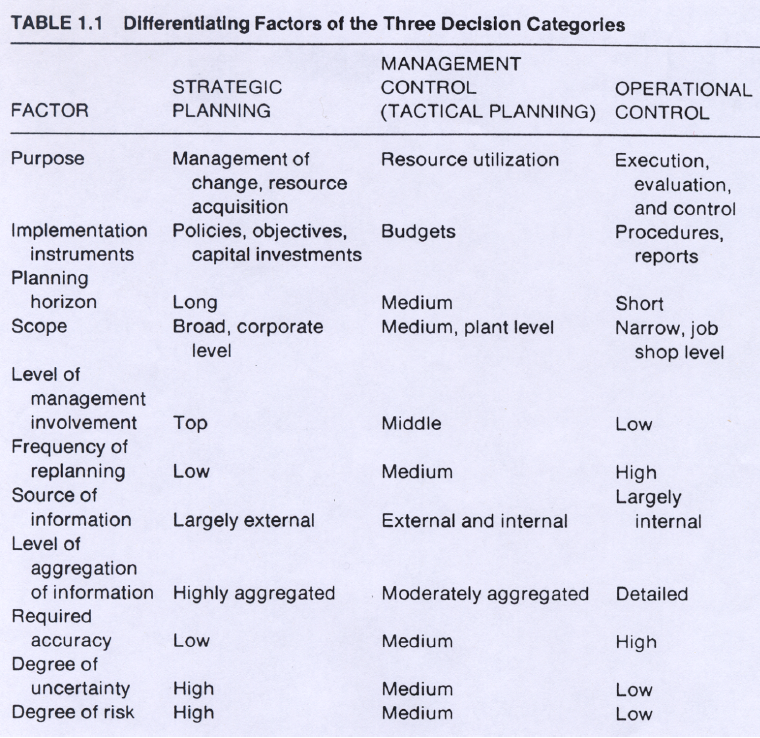
\includegraphics[width=150px]{img/OMEntscheidungsebene.png}
	\captionof{figure}{Entscheidungsebene im OM}
	\label{fig:Entscheidungsebene im OM}
\end{Figure}

\textbf{Entscheidungselemente}
\begin{itemize}
   \item Produkte
   \item Potentiale (Kapazitäten)
   \item Prozesse
\end{itemize}

\begin{Figure}
\centering
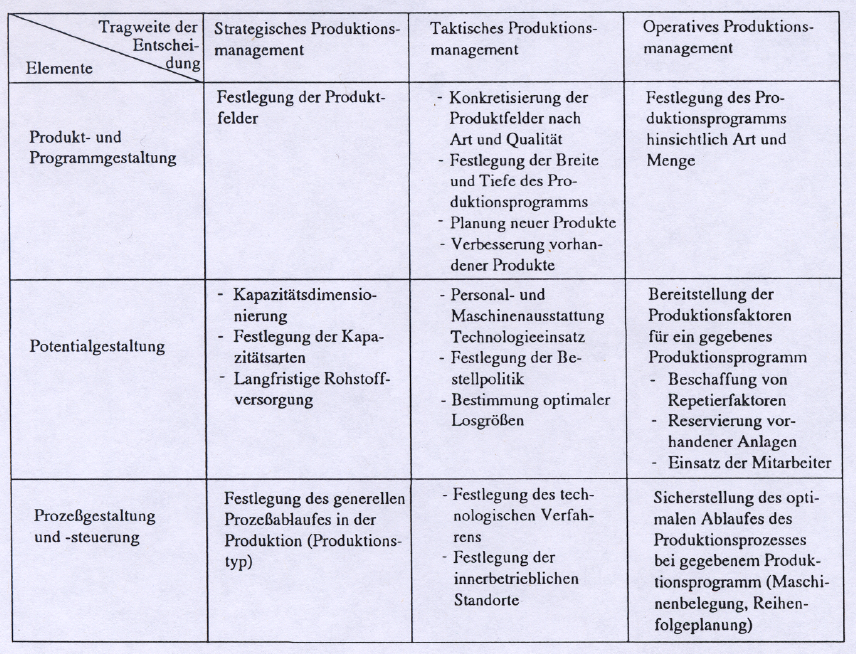
\includegraphics[width=150px]{img/OMEntscheidungselemente.png}
	\captionof{figure}{Entscheidungselemente im OM}
	\label{fig:Entscheidungselemente im OM}
\end{Figure}


   \subsection{Unternehmenstrategie}
Wird grundsätzlich in die vier Bereiche unterteilt:
\begin{itemize}
   \item Quality
   \item Costs
   \item Delivery
   \item Flexibility
\end{itemize}
Diese vier Bereiche stehen natürlich in einem gewissen Masse in einem Zielkonflikt. Da sehr hohe Qualität sehr selten mit sehr niedrigen Kosten hereingehen usw.

\section{Arbeitsdefinitionen}

\textbf{System}
\begin{itemize}
   \item Menge von Objekten (Entitäten, Systemelementen), welche zu einem bestimmten Zweck miteinander verbunden sind und gegenseitig interagieren
   \item Beschreibung eines Systems oft anhand eines (evtl. zeitabhängigen) Systemzustands
   \item \textit{Systemanalyse} Eher statische (zeitunabhängige) Betrachungsweise: 'Was sind die Systemelemente, wie sind sie miteinander verbunden und wie interagieren sie?
\end{itemize}

\textbf{Prozess}
\begin{itemize}
   \item Ablauf einer Folge von zusammenhängenden Aktionen (Aktivitäten, Operationen, Handlungen,...)
   \item Folge von Zustandsänderungen eines Systems
   \item \textit{Prozessanalyse:} Eher dynamisch (zeitabhängige) betrachtet: 'Was sind die zeitlichen Abläufe / Handlungsfolgen bzw. die zeiitlichen Veränderungen des Systemzustands?'
\end{itemize}

\textbf{Planung}
\begin{itemize}
   \item Plan: Handlungsabsicht, gedankliche Vorwegnahme zukünftiger Handlungen
   \item Planung: Entwicklung eines Plans (zukunftsgerichtet): Festlegen von Zielen (Sollwerten) und von Methoden zur Erreichung dieser Ziele
\end{itemize}

\textbf{Steuerung}
\begin{itemize}
   \item Umsetzungeines Plans (gegenwartsbezogen): Veranlassung von Handlungen, Kontrolle von ISTwerten gegenüber SOLLwerten, Anpassung des Plans ('Regelkreis')
\end{itemize}


\chapter{Einführung in die Prozess-Analyse}

\section{Qualitative Prozessanalyse}
Für die qualitative Prozessanalyse gibt es eine Vielzahl an Notationen (bspw. BPM), Begrifflichkeiter, jedoch \textbf{keine} klare einheitliche bzw. normierte Terminologie.\\
Wobei der Begriff \textit{Business Process} ein betrieblicher Ablauf darstellt:
\begin{itemize}
   \item Menge von Teilprozessen (Aktivitäten, Vorgängen, Aktionen, Tätigkeiten, ...), welche in bestimmten logischen und zeitlichen Zusammenhang stehen
   \item \textbf{EN Definition:} \textit{A business process is a colleciton of interrelated work tasks, initiated in response to an event, that achieves a specific result for the customer of the process}
\end{itemize}

\textbf{Ziele:}
\begin{itemize}
   \item Analyse bestehender Prozesse ('As-Is') $\rightarrow$ identifizieren, Verstehen, Dokumentieren
   Verbesserung bestehender Prozesse, Gestaltung neuer Prozesse ('To-Be') $\rightarrow$ Aufdecken von Optimierungspotential, Umsetzung in neue Abläufe
\end{itemize}

\textbf{Methodik:}
\begin{itemize}
   \item[i] Sprachliche Beschreibung der Prozesse
   \item[ii] Graphische Darstellung in Form von Prozessdiagrammen 
\end{itemize}

   \subsection{Grundlagen der Prozessdiagramme}
Prozessdiagramme sind eine grafische Darstellung eines Prozesses, welche Teilprozesse und deren Zusammenhänge abbilden (bspw. mit Symbole und Pfeile)\\
Für diese grafische Darstellung gibt es viele unterschiedliche notationen (bspw. Anzahl Symbole, Pfeiltypen, Ziel, Spezifikation). Es ist elementar diese Notation zu verstehen, damit man das Diagramm korrekt liest, 
ansonsten können missinterpretationen folgen. Beispiele von unterschiedlichen Arten:
\begin{itemize}
   \item Hierarchische Strukturierung von Prozessen $\rightarrow$ Baukasten-System, Detailgrad abhängig von Anwendung und Zielsetzung
   \item Questions and Facts (bspw. IT-Anwendung)
   \item nesting structure
\end{itemize}

\begin{Figure}
\centering
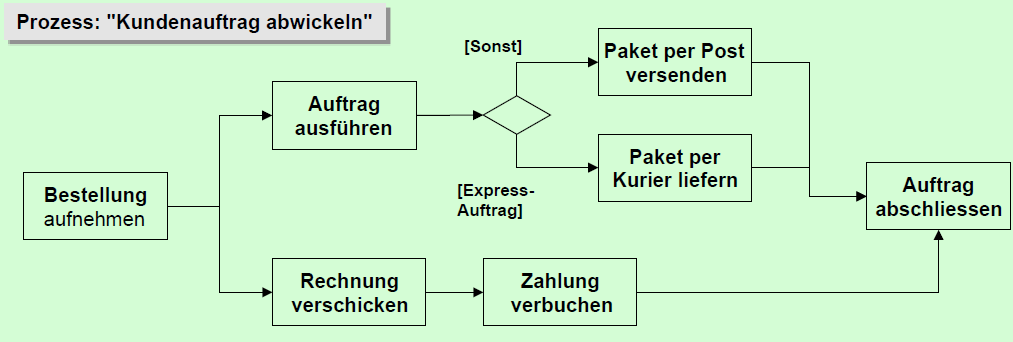
\includegraphics[width=150px]{img/BspProzessdiagramm.png}
	\captionof{figure}{Beispiel eines Prozessdiagrammes für die Kundenauftrag Abwicklung}
	\label{fig:Beispiel eines Prozessdiagrammes für die Kundenauftrag Abwicklung}
\end{Figure}

      \subsubsection{Prozessdiagramm-Typen}
$\rightarrow$ Es gibt zahlreiche Diagrammsprachen (Modellierungssprachen).

\textbf{Definition:}
\begin{itemize}
   \item \textbf{Syntax:} \textit{Konstruktionsregeln für zulässige Diagramme (Symbole, Verbindungen, ...)}
   \item \textbf{Semantik:} \textit{Erklärung der Bedeutung (Interpretation) der verschiedenen Sprachelemente}
   \item $\rightarrow$ In der Praxis häufig nicht formal exakt definiert
\end{itemize}

 \textbf{elementare Grundtypen:} $\rightarrow$ Unterscheidung bezüglich Interpretation der Pfeile\\
 \textit{Aktivitätsdiagramme} (Activity Diagrams, Workflow Diagrams, ...):\\
 $\rightarrow$ Pfeil bedeutet Zeitliche Präzedenz (genauer 'Sequenzfluss') 
 \begin{Figure}
\centering
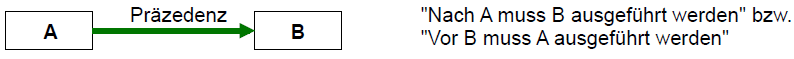
\includegraphics[width=150px]{img/Praezedenzfluss.png}
	\captionof{figure}{Beispiel eines Aktivitätsdiagramme}
	\label{fig:Beispiel eines Aktivitätsdiagramme}
\end{Figure}

\textit{Flussdiagramme} (Flow Diagram, Material Flow Diagram, ...):\\
$\rightarrow$ Pfeil bedeutet Fluss von OBjekten von A nach B (Material, Aufträge, ...)
 \begin{Figure}
\centering
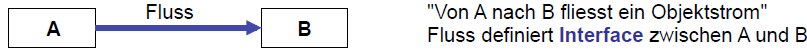
\includegraphics[width=150px]{img/Fluss.png}
	\captionof{figure}{Beispiel eines Flussdiagramms}
	\label{fig:Beispiel eines Flussdiagramms}
\end{Figure}

      \subsubsection{Entwicklung von Prozessdiagramme}
\begin{itemize}
   \item \textbf{Wichtig:} Klare Zielsetzung/Fragestellung bei der Prozessanalyse
   \item Schwierigkeiten $\rightarrow$ Identifikation/Abgrenzung der Prozesss und Detaillierung/Verknüpfung der Subprozesse
   \item Erstellen von guten Diagrammen ist eine 'Kunst'
   \item Gefahr: Paralysis By Analysis $\rightarrow$ Zu hohe, unangemessene Ansprüche an Detaillierungsgrad $\Rightarrow$ Modellierung endlos
\end{itemize}

Hilfreiche Anwendungtipps:
\begin{itemize}
   \item Detail nur soweit wie Zielsetzung
   \item Diagramme so einfach wie möglich halten
   \item Diagramme sollten möglichst selbsterklärend sein
\end{itemize}

   \subsection{Aktivitätsdiagramme}
      \subsubsection{Syntax}

\begin{Figure}
\centering
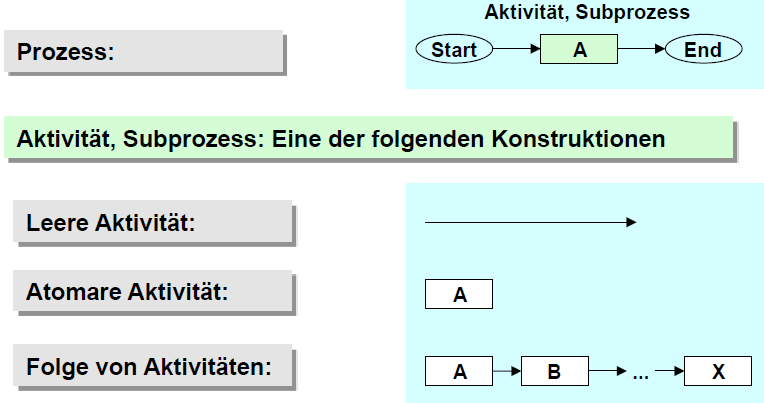
\includegraphics[width=200px]{img/AkDiaSyntaxI.png}
	\captionof{figure}{Syntax der Aktivitätsdiagramme}
	\label{fig:Syntax der Aktivitätsdiagramme}
\end{Figure}

\begin{Figure}
\centering
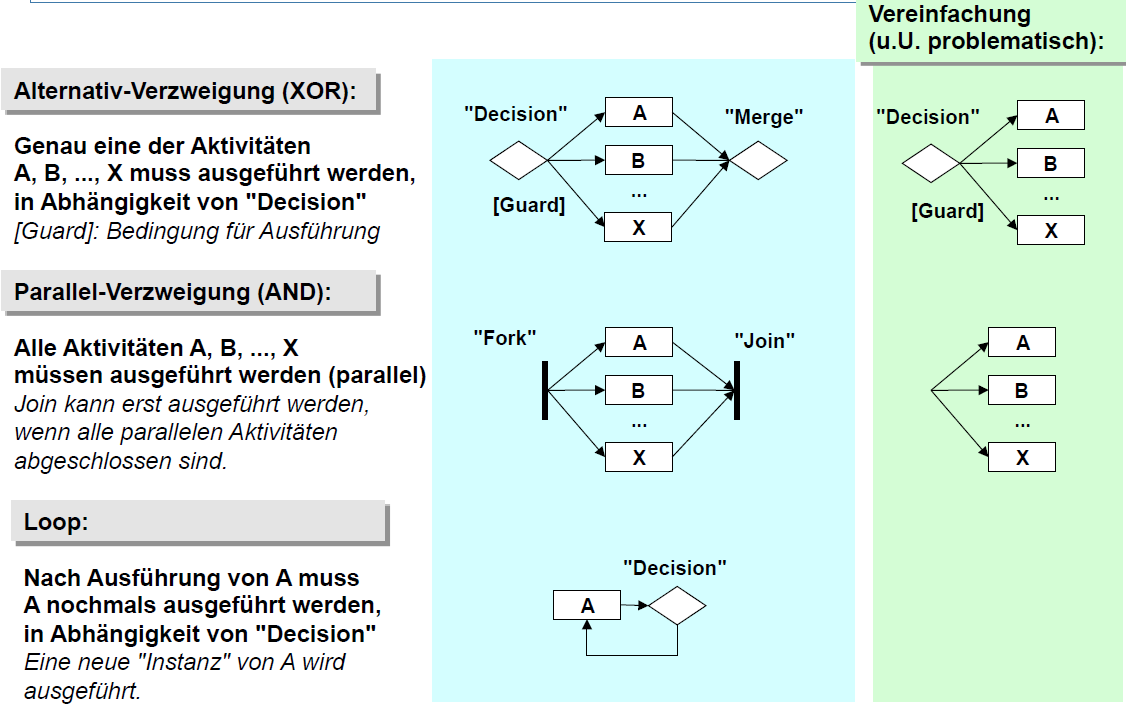
\includegraphics[width=200px]{img/AkDiaSyntaxII.png}
	\captionof{figure}{Syntax der Aktivitätsdiagramme II}
	\label{fig:Syntax der Aktivitätsdiagramme II}
\end{Figure}

\begin{Figure}
\centering
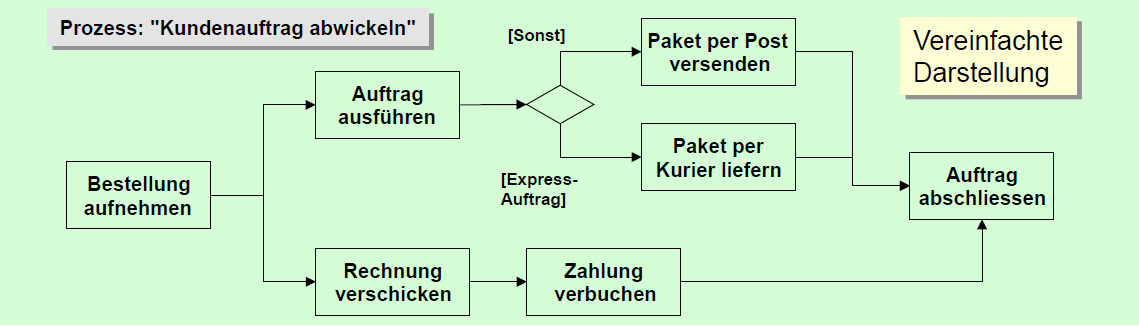
\includegraphics[width=150px]{img/AkDiaVereinfacht.png}
	\captionof{figure}{Vereinfachte Darstellung eines Aktivitätsdigramm für den Kundenauftrag abwickeln}
	\label{fig:Vereinfachte Darstellung eines Aktivitätsdigramm für den Kundenauftrag abwickeln}
\end{Figure}

\begin{Figure}
\centering
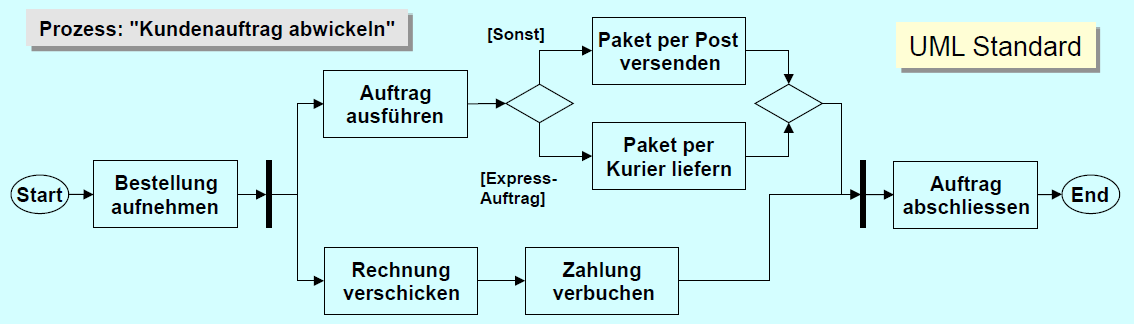
\includegraphics[width=150px]{img/AkDiaUML.png}
	\captionof{figure}{UML Darstellung eines Aktivitätsdigramm für den Kundenauftrag abwickeln}
	\label{fig:UML Darstellung eines Aktivitätsdigramm für den Kundenauftrag abwickeln}
\end{Figure}

\begin{Figure}
\centering
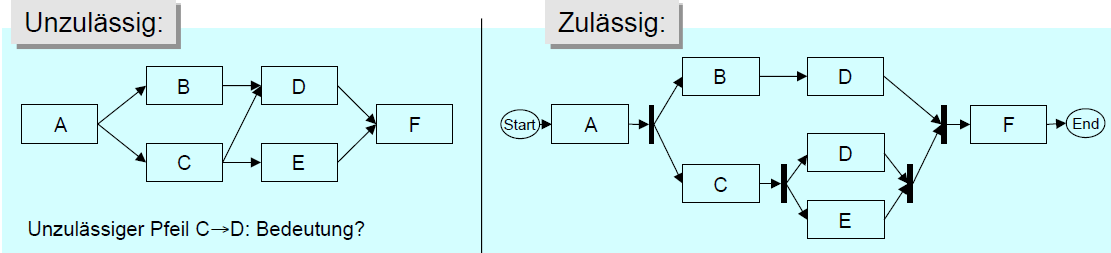
\includegraphics[width=150px]{img/AkDiaDoDonts.png}
	\captionof{figure}{un- bzw zulässig eines Aktivitätsdigramm}
	\label{fig:un- bzw zulässig eines Aktivitätsdigramm}
\end{Figure}

      \subsubsection{Semantik}
Jeder \textit{Weg} (Routing) vom Start- zum Endkonoten beschreibt möglichen \textit{Verlauf} des Prozesses


   \subsection{Swimlane-Diagramme}
Gilt als Erweiterung der Aktivitäts-Diagramme - wobei eine zusätzliche Information (der Akteur / die Rolle) ersichtlich ist $\rightarrow$ \textit{Wer führt eine Aktivität durch (oder: ist zuständig dafür...)}\\
\textbf{ohne Swimlane:} \textit{Was wird in welcher Reihenfolge ausgeführt?}\\
\textbf{mit Swimlane:} \textit{Was wird von wem in welcher Reihenfolge ausgeführt?}\\
\textbf{typische Akteure:} Person, Personengruppe, Jobfunktion, Organisationseinheit, Maschine, Einrichtung, Computer

\begin{Figure}
\centering
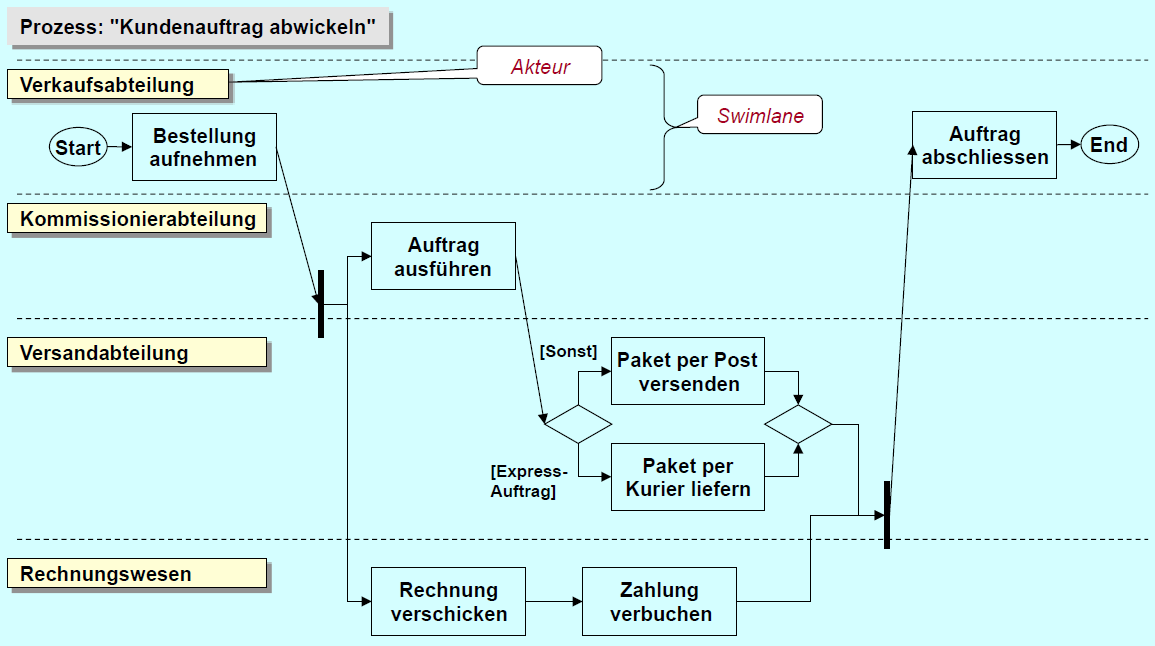
\includegraphics[width=150px]{img/BspSwimlane.png}
	\captionof{figure}{Beispiel eines Swimlane-Diagramm}
	\label{fig:Beispiel eines Swimlane-Diagramm}
\end{Figure}

   \subsection{Flussdiagramme}
\textbf{wichtig!} Keine normierte Terminologie\\

      \subsubsection{Semantik}
\begin{itemize}
   \item Pfeile stellen Flüsse von Objekten dar (Material, Aufträge, ...)
   \item Flüsse definieren Schnittstellen zwischen Subprozessen (Aktivitäten): Input, Output
   \item Flussobjekte werden im Subprozess transformiert (Physikalisch, örtlich, zeitlich)
\end{itemize}

      \subsubsection{Syntax}
Für jeden Flusstyp, d.h. jede unterschiedlcihe Art von Flussobjekten: Diagramm bildet ein sogenanntes \textbf{S-T-Netzwerk}:
\begin{itemize}
   \item zusammenhängendener Graph (Knoten: Aktivitäten, Pfeile: Flüsse)
   \item Genau ein Startknoten: \textbf{Quelle (S: Source)} $\rightarrow$ generiert FLussobjekte, nur austretende Pfeile
   \item Genau ein Endknoten: \textbf{Senke (T: Target)} $\rightarrow$ konsumiert Flussobjekte, nur eintretende Pfeile
   \item Alle anderen Zwischenknoten brauchen mind. 1 ein- und 1 austretender Pfeil
   \item Manchmal werden Quelle und Senke auch weggelassen
\end{itemize}

      \subsubsection{Unterschied zu Aktivitätsdiagrammen}
\begin{itemize}
   \item Keine Parallelverzweigung
   \item Jede Verzweigung ist eine Alternativ-Verzweigung $\rightarrow$ Bei Verzweigung häufig Prozentangabe für Flussanteil
   \item \textbf{Routing} Möglicher Weg eines Flussobjekts von der Quelle zur Senke 
\end{itemize}

\begin{Figure}
\centering
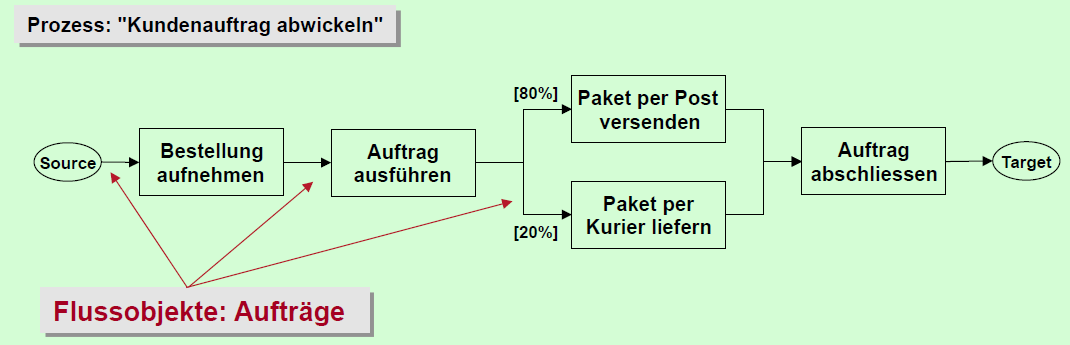
\includegraphics[width=150px]{img/BspFlussdiagramm.png}
	\captionof{figure}{Beispiel eines Flussdiagramm}
	\label{fig:Beispiel eines Flussdiagramm}
\end{Figure}

      \subsubsection{Zu beachten}
\begin{itemize}
   \item Immer Typ (Auftrag, Komponente, Gewichtseinheiten, ...) und Masseinheit (Anzahl, Kg, Stunden, ...) der Flussobjekte spezifzieren
   \item Flüsse verschiedener Objekttypen/-einheiten können nicht zusammengeführt werden
   \item vers. Flusstypen im gleichen Diagramm graphisch unterscheiden (bspw. vers. Pfeildarstellung)
\end{itemize}

\begin{Figure}
\centering
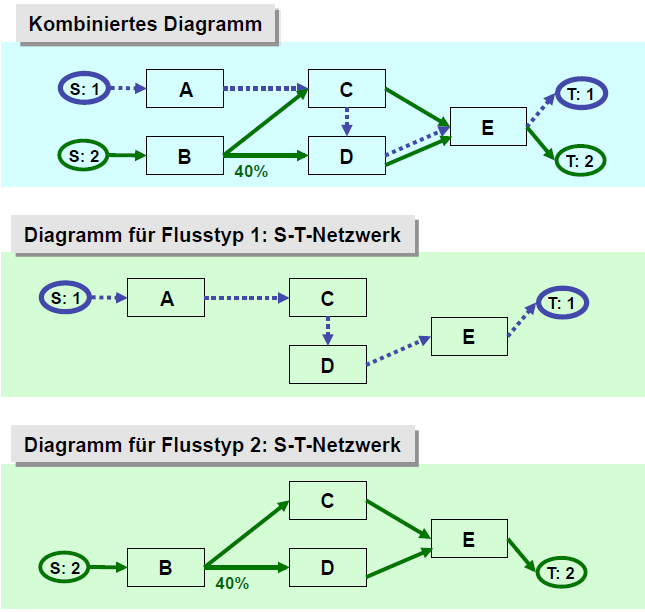
\includegraphics[width=150px]{img/BspFlussdiagrammZweiTypen.png}
	\captionof{figure}{Beispiel eines Flussdiagramm mit zwei Flusstypen}
	\label{fig:Beispiel eines Flussdiagramm mit zwei Flusstypen}
\end{Figure}

      \subsubsection{Puffer}
\begin{itemize}
   \item Puffer sind spezielle Subprozesse (Aktivitäten), welche zur 'zeitlichen Transformation' (Lagerung) dienen ($\rightarrow$ Zwischenspeicher, Lager, Warteraum etc)
   \item da spezielle Bedeutung häufig eigenes Symbole
   \item Mehrstufige Prozesse sind häufig gepuffert
   \item Dienen dazu \textbf{Blocking} (Blockierung) und \textbf{Starving} (Aushungern) zu vermeiden
\end{itemize}

   \subsection{UML und Standards}

      \subsubsection{einige Standards}
\begin{itemize}
   \item Integrated DEFinition $\rightarrow$ IDEF $\Rightarrow$ Sammlung verschiedener Modellierungssprachen
   \item Business Process Modeling Notation $\rightarrow$ BPMN 
   \item Unified Modeling Language $\rightarrow$ UML $\Rightarrow$ Standard in Software-Entwicklung; Sammlung von zahlreichen versch. Diagrammtypen inkl. Spezifikation
\end{itemize}

      \subsubsection{UML}
In UML sind folgende Diagramme am wichtigsten:

\begin{Figure}
\centering
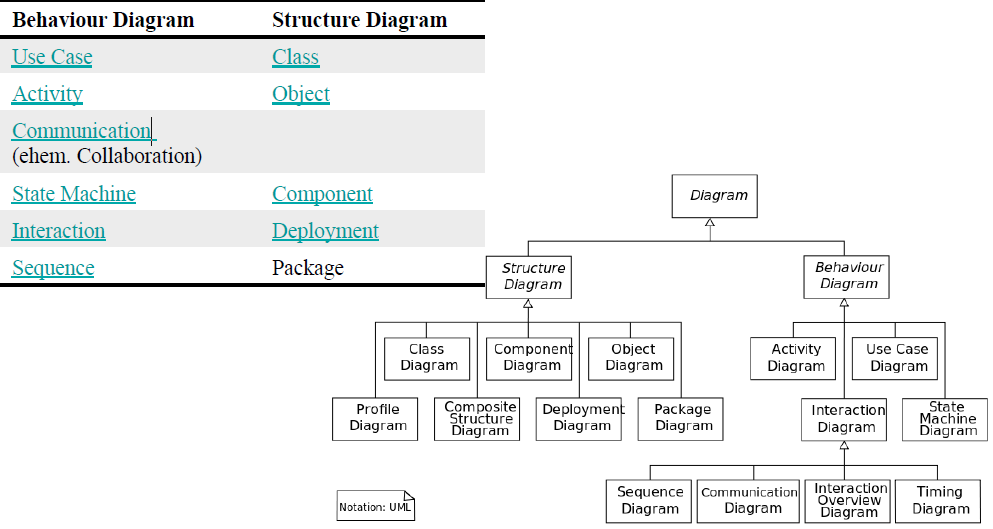
\includegraphics[width=150px]{img/TopOfUML.png}
	\captionof{figure}{Übersicht der wichtigsten UML Diagramme}
	\label{fig:Übersicht der wichtigsten UML Diagramme}
\end{Figure}

\textbf{Object Diagram}
\begin{Figure}
\centering
\includegraphics[width=150px]{img/ObjectDiagram.png}
	\captionof{figure}{Object Diagram nach UML}
	\label{fig:Beispiel eines Object Diagram nach UML}
\end{Figure}

\textbf{Class Diagram}
\begin{Figure}
\centering
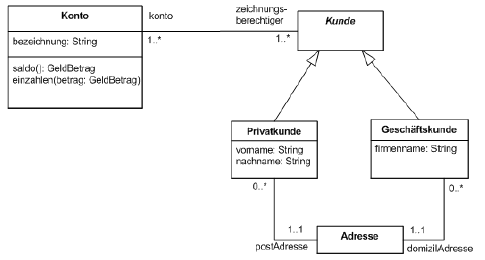
\includegraphics[width=150px]{img/ClassDiagram.png}
	\captionof{figure}{Class Diagram nach UML}
	\label{fig:Beispiel eines Class Diagram nach UML}
\end{Figure}

\textbf{Sequence Diagram}
\begin{Figure}
\centering
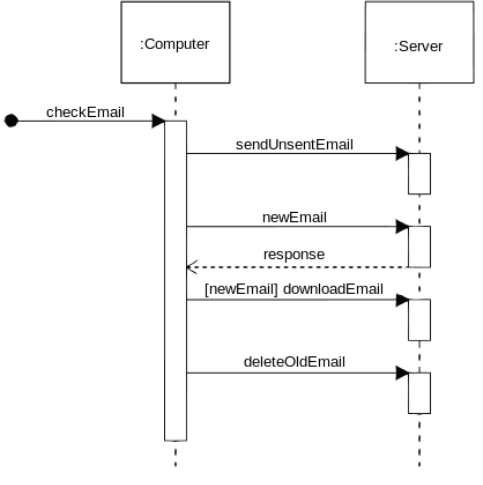
\includegraphics[width=150px]{img/SequenceDiagramm.png}
	\captionof{figure}{Sequence Diagram nach UML}
	\label{fig:Beispiel eines Sequence Diagram nach UML}
\end{Figure}

\textbf{Activity Diagram}
\begin{Figure}
\centering
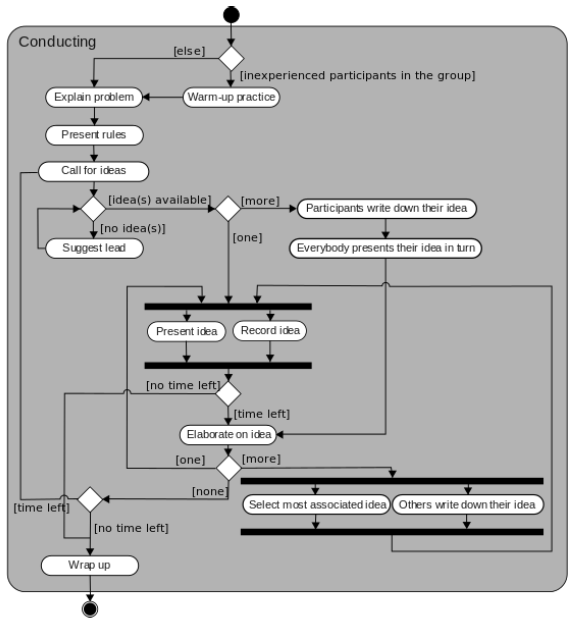
\includegraphics[width=150px]{img/ActivityDiagram.png}
	\captionof{figure}{Activity Diagram nach UML}
	\label{fig:Beispiel eines Activity Diagram nach UML}
\end{Figure}

\textbf{UseCase Diagram}
\begin{Figure}
\centering
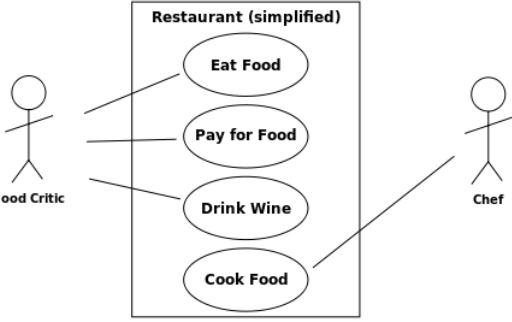
\includegraphics[width=150px]{img/UseCaseDiagram.png}
	\captionof{figure}{UseCase Diagram nach UML}
	\label{fig:Beispiel eines UseCase Diagram nach UML}
\end{Figure}

\textbf{State Machine Diagram}
\begin{Figure}
\centering
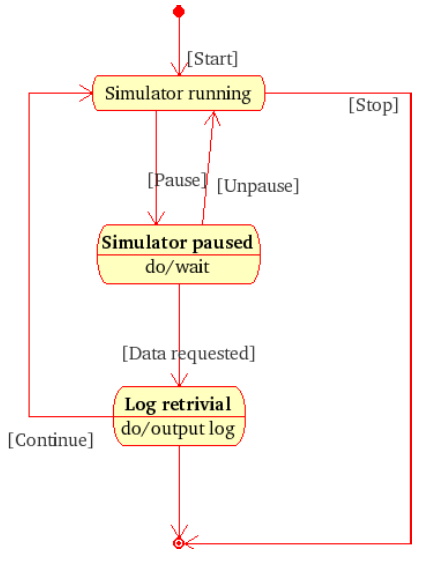
\includegraphics[width=150px]{img/SMDiagram.png}
	\captionof{figure}{State Machine Diagram nach UML}
	\label{fig:Beispiel eines State Machine Diagram nach UML}
\end{Figure}

\textbf{Communication Diagram}
\begin{Figure}
\centering
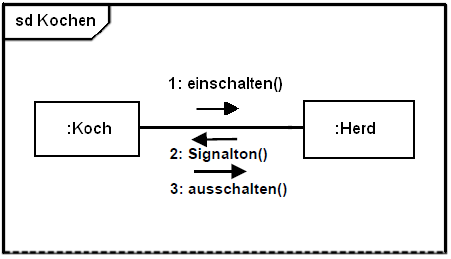
\includegraphics[width=150px]{img/CommunicationDiagram.png}
	\captionof{figure}{Communication Diagram nach UML}
	\label{fig:Beispiel eines Communication Diagram nach UML}
\end{Figure}

\textbf{Interaction Diagram}
\begin{Figure}
\centering
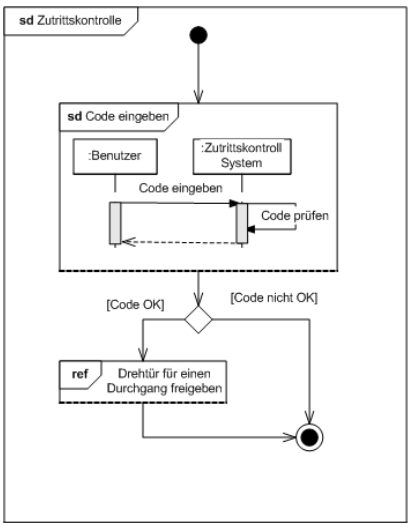
\includegraphics[width=150px]{img/InteractionDiagram.png}
	\captionof{figure}{Interaction Diagram nach UML}
	\label{fig:Beispiel eines Interaction Diagram nach UML}
\end{Figure}

\textbf{Deployment Diagram}
\begin{Figure}
\centering
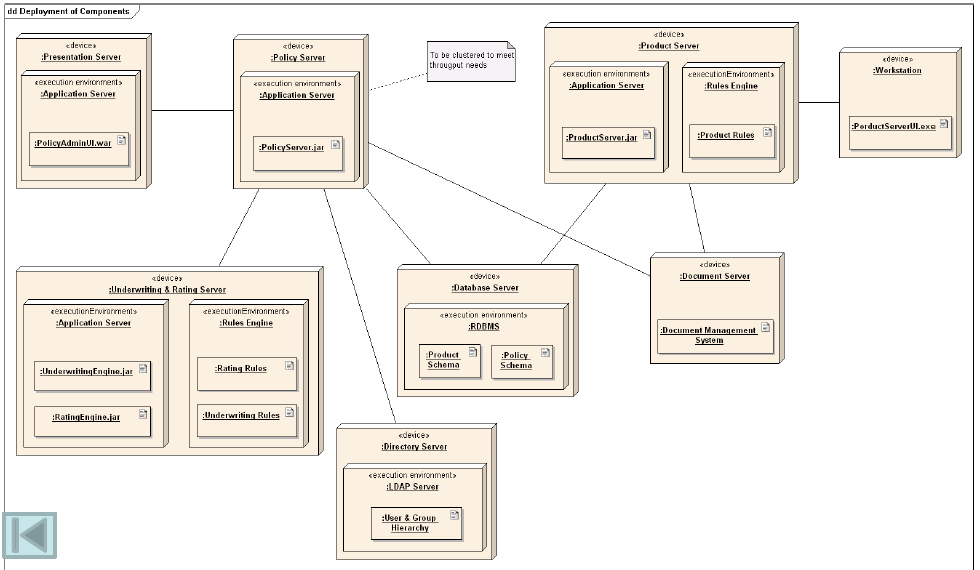
\includegraphics[width=150px]{img/DeploymentDiagram.png}
	\captionof{figure}{Deployment Diagram nach UML}
	\label{fig:Beispiel eines Deployment Diagram nach UML}
\end{Figure}

\textbf{Component Diagram}
\begin{Figure}
\centering
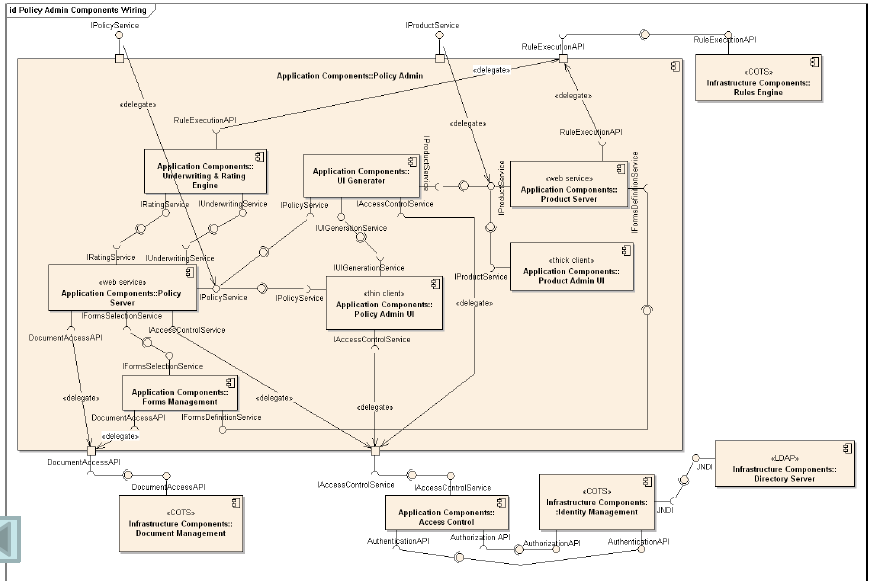
\includegraphics[width=150px]{img/ComponentDiagram.png}
	\captionof{figure}{Component Diagram nach UML}
	\label{fig:Beispiel eines Component Diagram nach UML}
\end{Figure}

\textbf{Package Diagram}
\begin{Figure}
\centering
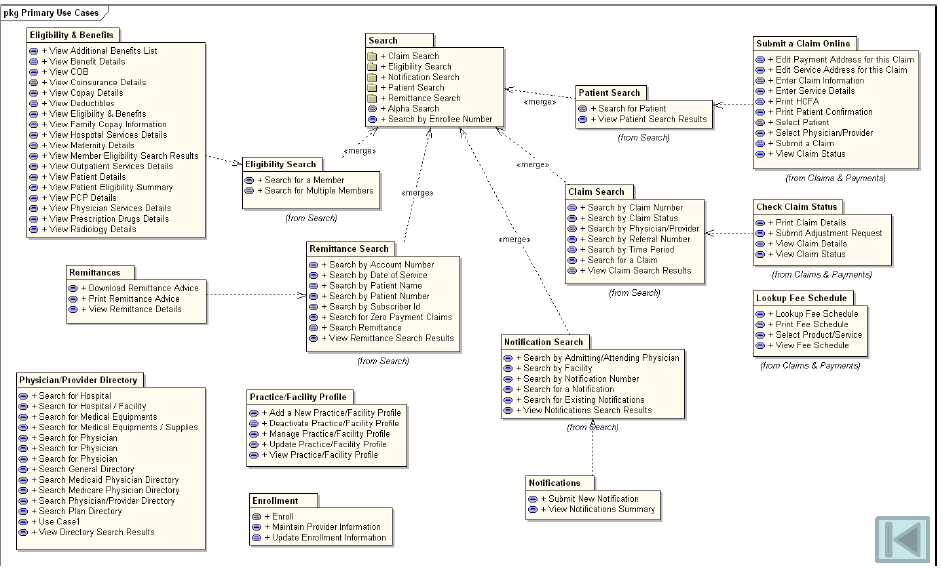
\includegraphics[width=150px]{img/PackageDiagram.png}
	\captionof{figure}{Package Diagram nach UML}
	\label{fig:Beispiel eines Package Diagram nach UML}
\end{Figure}

\section{Quantitative Prozessanalyse}

   \subsection{Formel von Little}
Betrachte einzelnen Prozess (Subprozess) als Blackbox, welche Input zu Output transformiert ($\rightarrow$ Transformationsprozess).\\
Annahme: Nur ein Typ von Flussobjekten (Flusseinheit) fliesst durch den Prozess.
\begin{Figure}
\centering
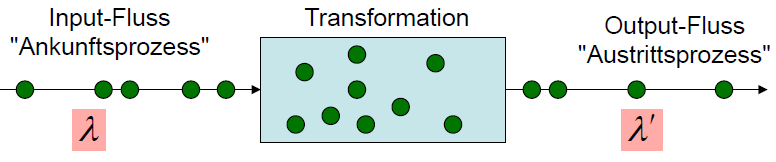
\includegraphics[width=150px]{img/BlackboxVonLittle.png}
	\captionof{figure}{Abbildung des Flusses nach Little}
	\label{fig:Abbildung des Flusses nach Little}
\end{Figure}

      \subsubsection{Gleichgewichtsbedingung}
Ein Prozess ('System') ist im \textbf{Gleichgewicht} ('stabil') wenn $\lambda = \lambda'$ gilt.\\
Wobei $\frac{1}{\lambda}$ die mittlere Zwischenankunftszeit beschreibt
\begin{Figure}
\centering
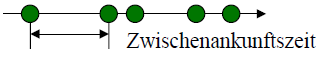
\includegraphics[width=150px]{img/Zwischenankunftszeit.png}
	\captionof{figure}{Abbildung der Zwischenankunftszeit}
	\label{fig:Abbildung der Zwischenankunftszeit}
\end{Figure}

      \subsubsection{Die 3 zentralen Leistungskennzahlen eines (stabilen) Prozesses}
$\lambda$, $\lambda '$: mittlere Ankunfts-/Austrittsrate ('mean arrival / exit rate') $\Rightarrow$ $\frac{Anzahl eintretende / austretende Flusseinheit}{Zeiteinheit}$ in der Masseinheit [FE/ZE]\\
$N$: mittlere Anzahl Objekte im System ('mean number of objects in system') in der Masseinheit [FE]\\
$W$: mittlere Aufenthaltszeit eines Objekts im System ('mean sojourn time') in der Masseinheit [ZE]\\

Wobei \textit{mittlere} über langen Zeitraum bedeutet.

\begin{Figure}
\centering
\includegraphics[width=150px]{img/stabilderProzess.png}
	\captionof{figure}{Abbildung eines stabilen Prozesses}
	\label{fig:Abbildung eines stabilen Prozesses}
\end{Figure}

      \subsubsection{Die Formeln}
In der quantitative Prozessanalyse ist die Formel von Little ein fundamentaler Zusammenhang, welcher unter sehr allgemeinen Bedingungen gültig ist. Es wird auch das Ohmsche Gesetz in der Prozessanalyse genannt.
\begin{equation}
   N = \lambda * W
\end{equation}

Doch auch im Operations Management hat es eine wichtige Bedeutung:
\begin{equation}
   WIP = TH * CT
\end{equation}

WIP: (mean) Work in Process $\rightarrow$ mittlere Ware-In-Arbeit ('WIA')\\
TH: (mean) Throughput $\rightarrow$ mittlerer Durchsatz, mittlere Produktionsrate\\
CT: (mean) Cycle Time $\rightarrow$ mittlere Durchlaufzeit ('DLZ')\\
\\
\textbf{Anwendung in Operations Management}\\
\begin{itemize}
   \item Anwendbar auf bel. Prozesse (Bereiche) in einem Betrieb $\rightarrow$ Ganzer Betrieb, Teilbetrieb, Arbeitsstation, Arbeitsplatz, Bedienschalter, Maschine, ...
   \item Allgemeine relation zwischen den 3 Kenngrössen (WIP, TH, CT) $\rightarrow$ Falls zwei Grössen bekannt sind, kann dritte Grösse berechnet werden
   \item Reduktion von Durchlaufzeiten (bei konstanter Produktionsrate) $\rightarrow$ DLZ wächst/sinkt proportional zu WIA $CT = \frac{1}{TH}* WIP$
   \item Ermittlung Durchlaufzeit in Praxis $\rightarrow$ DLZ ist sehr aufwendig zu messen, jedoch lässt sich dies durch die beiden anderen Kenngrössen WIP und Produktionsrate ermitterln $CT = \frac{WIP}{TH}$
   \item Messung der WIP in Form von Zeitaufwand $\rightarrow$ Little's Formel kann als Umrechnung der Masseinheit WIP gesehen werden
\end{itemize}

   \subsection{Kapazität und Auslastung, Bottleneck}

      \subsubsection{Begriff der Kapazität}
\begin{itemize}
   \item Kapazität als mengemässiges Leistungsvermögen, welches immer bezüglich eines \textbf{enzigen Objekttyps (Produkts)} gemessen wird.\\
   \item \textbf{Definition:} \textit{Kapazität einer Ressource (eines Prozesses) bezüglich eines bestimmten Objekttypes (Produkts): Die maximal mögliche Ausbringsungsmenge (Output) fpr diesen Objekttyp (Produkt) in einem bestimmten Zeitraum}\\
   \item Kapazität $\mu$ = maximal möglicher (mittlerer) Throughput 
   \item Masseinheit: [Anzahl Objekte / Zeiteinheit]
   \item per Definition gilt $\lambda \leq \mu$ bzw. TH $\leq \mu$ $\Rightarrow$ $\lambda$ = TH die Ankrunftstrate bzw. den Throughput bezeichnet
   \item minimale (mittlere) Aufenthaltsdauer ('mittlere Bearbeitungszeit') = $\frac{1}{\mu}$
   \item Falls mehrere Objekttypen $i \in I$ durch einen Prozess fliessen $\rightarrow$ Kapazität $\mu_i =$ maximal möglicher mittlerer Throughput bzgl. $i$
\end{itemize}

      \subsubsection{Begriff der Auslastung}
\begin{itemize}
   \item Auch Auslastungsgrad, Kapazitätsauslastungsgrad genannt
   \item Auslastung einer Ressource (Prozesses): Auslastung = $\frac{Genutze Kapazität}{Nutzbare Kapazität}$
   \item Masseinheit: einheitslos (bspw. \%)
   \item \textbf{Bottleneck} eines Routings:Teilprozess mit grösster Auslastung
   \item Auslastung p = $\frac{\lambda}{\mu}$ = $\frac{Throughput}{Nutzbare Kapazität}$ wobei immer $p > 1$ gilt
   \item bei mehreren Objekttypen $i \in I$: Auslastung bzgl. Objekttyp (Produkt) i $p_i = \frac{\lambda_i}{\mu_i}$
   \item bei mehreren Objekttypen $i \in I$: Gesamtauslastung $p = \sum_{i \in I} p_i$
\end{itemize}


\chapter{Elemente der Warteschlangentheorie}

\section{Einführung und Grundlage}
In Operations Management geht es darum die Ressourcen so dimensionieren, dass
\begin{itemize}
   \item Warteschlange klein, bzw. selten sind, ein Kunde im MIttel wenig wartet, ein gewisser \textit{Servicegrad} gesichert ist
   \item Ein \textit{Kostenoptimum} erzielt wird
\end{itemize}
$\rightarrow$ wird auch als Wartephänomen zusammengefasst, welches in OM allgegenwertig ist

\begin{Figure}
\centering
\includegraphics[width=150px]{img/Kostenoptimum.png}
	\captionof{figure}{Abbildung eines Kostenoptimum}
	\label{fig:Abbildung eines Kostenoptimum}
\end{Figure}

\begin{itemize}
   \item Warteschlangenphänomene entstehen mit dem Verbrauch von beschränkten Ressourcen
   \item Ressource (physisch, logisch, menschlich) wird benötigt um Tätigkeit an Entitäten auszuführen, welche allgemein mit \textit{Kunden} bezeichnet werden
   \item Auch wenn im Mittel genügend Ressourcen vorhanden, können Konflikte entstehen $\rightarrow$ Wartephänomene für Kunden
   \item Warteschlangenphänomene können quantiativ untersucht werden (einfachen Fälle: Queueing Theorie; komplexe Fälle: Simulationsmodelle) $\Rightarrow$ Bei beidem handelt es sich um stoachastische Modelle, d.h. gewisse Daten sind vom Zufall bestimmt und man will sie als Zufallsvariablen Modellierungssprachen
   \item Beide sind Modelle, die zeitliche Prozesse beschreiben 
   \item Queueing Theorie ist das analytische Werkezug für die Modellierung
\end{itemize}


   \subsection{Grundbegriffe der Warteschlangentheorie}
Eine Wartschlange ('Queue') ist ein stoachastisches (= zufälliges) System, das sich aus folgenden schematischen Elementen zusammensetzt.
\begin{Figure}
\centering
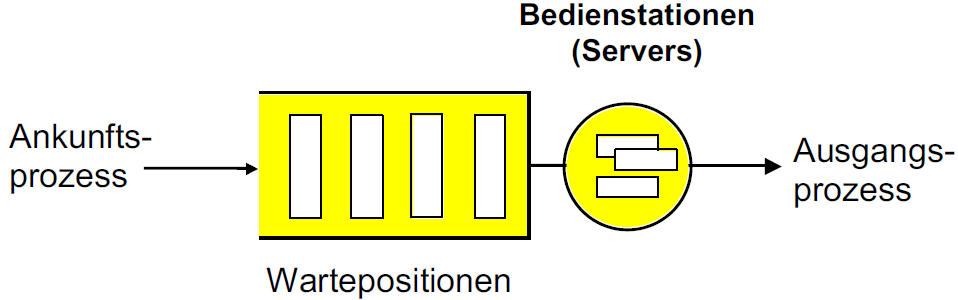
\includegraphics[width=150px]{img/Warteschlangentheorie.png}
	\captionof{figure}{Abbildung der Warteschlangentheorie}
	\label{fig:Abbildung der Warteschlangentheorie}
\end{Figure}

      \subsubsection{Ankunftsprozess}
\begin{itemize}
   \item Die Ankünfte der Kunden bilden einen stoachastischen Prozess $\rightarrow$ \textbf{Zwischenankunftszeit ('Interarrival Time', IAT)}
   \item Annahme: IAT ist unabhängig und gleichverteilt
   \item Notation \textbf{M}: Exponential-Verteilung (Markovian)
   \item Notation \textbf{D}: konstante Verteilung (Deterministic)
   \item Notation \textbf{G}: Beliebige Verteilung (General)
\end{itemize}

\begin{Figure}
\centering
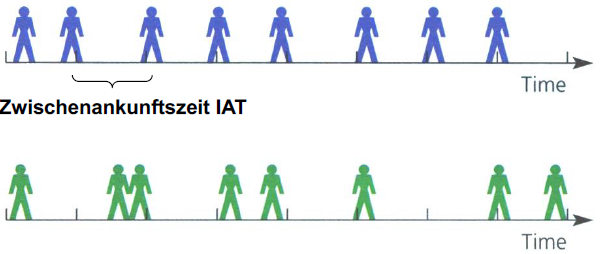
\includegraphics[width=150px]{img/IAT.png}
	\captionof{figure}{Abbildung der Zwischenankunftszeit}
	\label{fig:Abbildung der Zwischenankunftszeit}
\end{Figure}
Absolute Variabilität: Standardabweichung\\
Relative Variabilität: Variationskoeffizient (CV): $CV = \frac{Standardabweichung}{Erwartungswert}$

      \subsubsection{Warteschlangen-Disziplin}
Die Disziplin legt fest in welcher Reihenfolge der Zugriff stattfindet auf die Ressourcen\\
\textbf{FIFO bzw. FCFS} (First in, first out bzw. first come, first served) $\rightarrow$ Kunden werden in der Reihenfolge der Ankunft bedient. $\Rightarrow$ Allgemeines Default\\
\textbf{LIFO bzw. LCFS} (Last in, frist out bzw. last come, first served) $\rightarrow$ Kunden werdden in umgekehrter Reihenfolge der Ankunft bedient\\
\textbf{SIRO} (Service in random order) $\rightarrow$ Kunde wird zufällig aus der Wartschlange ausgewählt\\
\textbf{PS} (Processor Sharing) $\rightarrow$ Kunden teilen sich eine Bedienungsstelle. bei \textbf{n Kunden} erhält jeder $\frac{1}{n}$ der vorhandenen Ressourcen\\
\textbf{RR} (Round Robin) $\rightarrow$ Bedienung der Kunden im Kreis herum. Jeder erhält nacheinander ein Quantum $\sigma$. Falls noch mehr benötigt wird, stellt er sich wieder in die Warteschlange\\

Bei der \textbf{Preemption} werden die Kunden im Vorfeld nach Priorität in unterschiedlichen Klassen aufgeteilt.

      \subsubsection{Bedienung der Kunden}
Annahme: Die \textbf{Bedienzeit} (Service Time, ST) für die Bedienung eines Kunden sind unabhängige und gleichverteilte Zufallsvariablen.\\
Dabei entspricht die Anzahl Kunden, welche \textit{gleichzeitig} bedient werden können der \textbf{Anzahl Bedienstationen} der Warteschlange ($\rightarrow$ sämtliche Bedienstationen sind identisch)

      \subsubsection{Noation von Kendall}
Wartschlange wird mit einer symbolischen Formel beschrieben:
\textbf{A/B/s}\\
Wobei:\\
A $\rightarrow$ Verteilung der Zwischenankunftszeiten ($A \in [M,D,G]$)\\
B $\rightarrow$ Verteilung der Bedienzeiten ($B \in [M,D,G$])\\
s $\rightarrow$ Anzahl Bedienstationen ($s \in [1,2,..,n]$)\\

Folgende Annahmen gelten:
\begin{itemize}
   \item Die Menge (Population) der Klienten, welche in das System eintreten können, ist unbeschränkt
   \item die Anzahl der Klienten, welche sich inder Wartschlange befinden können, ist unbeschränkt
   \item die Wartschlangen-Disziplin ist FIO
\end{itemize}

\textbf{Erweiterte Form der Notation von Kendall} $\rightarrow$ A / B / s / K / P / DS\\
K $\rightarrow$ Kapazität der Warteschlange (Anzahl Warteplätze + Anzahl Bedienstationen)\\
P $\rightarrow$ Grösse der Population\\
DS $\rightarrow$ Warteschlangen-Disziplin\\

$\Rightarrow$ Fall einer beschränkten Kundenpopulation $\rightarrow$ Ankunftsprozess hängt von Anzahl Kunden im System abbilden\\
$\Rightarrow$ Fall einer beschränkten Aufnahmekapazität $\rightarrow$ Was passiert mit Ankommende, wenn Warteschlange voll ist? Kommen sie wieder oder nicht?

   \subsubsection{Leistungsmasse}
$N$ $\rightarrow$ Anzahl Kunden im System (an Warteposition oder in Bedienung)\\
$N_q$ $\rightarrow$ Anzahl Kunden in Warteschlange\\
$W$ $\rightarrow$ Aufenthaltszeit eines Kunden im System\\
$W_q$ $\rightarrow$ Wartezeit eines Kunden in Warteschlange\\
$\Rightarrow$ Diese Grössen sind Zufallsvariablen, deren Erwartungswert, Verteilung, Quantile (Schwellenwert) etc. abgeschätzt werden und sind im Allgemeinen von der Zeit \textit{t} abhängig. 
Für die Abschätzung ist es einfacher wenn das System sich in einem Gleichgewichtszustand befindet.

      \subsubsection{Beschreibende Parameter}
\begin{Figure}
\centering
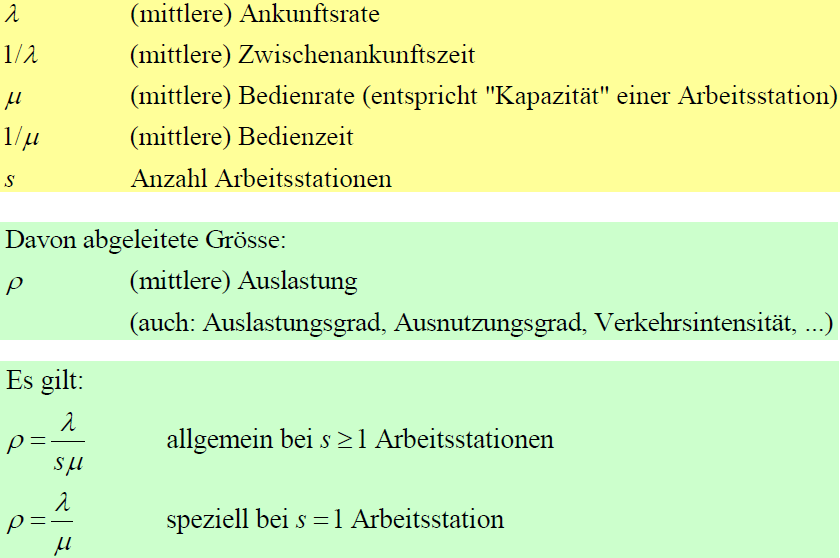
\includegraphics[width=150px]{img/BeschreibendeParamter.png}
	\captionof{figure}{Abbildung der beschreibenden Parameter}
	\label{fig:Abbildung der beschreibenden Parameter}
\end{Figure}

      \subsubsection{Leistungskennzahlen}
\begin{Figure}
\centering
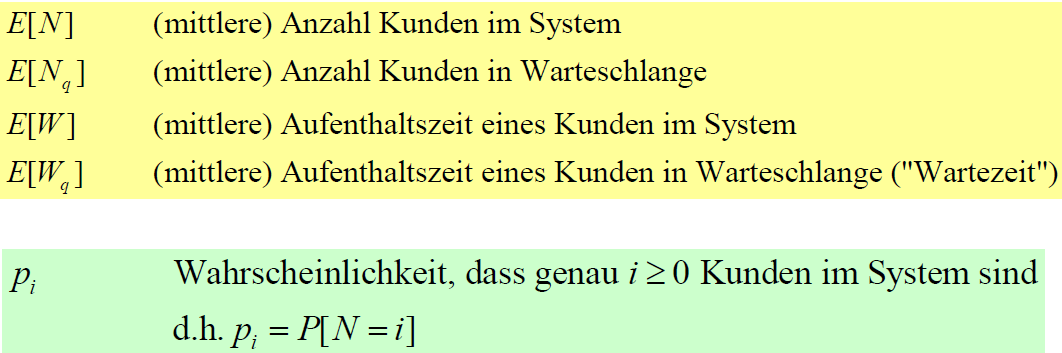
\includegraphics[width=150px]{img/Leistungskennzahlen.png}
	\captionof{figure}{Abbildung der Leistungskennzahlen}
	\label{fig:Abbildung der Leistungskennzahlen}
\end{Figure}

   \subsubsection{Grundlegende Zusammenhänge}
\begin{Figure}
\centering
\includegraphics[width=150px]{img/GrundlegendeZusammenhänge.png}
	\captionof{figure}{Abbildung der grundlegende Zusammenhänge}
	\label{fig:Abbildung der grundlegende Zusammenhänge}
\end{Figure}
$\rightarrow$ Falls E[N] gegeben ist, können die anderen drei Leistungsmasse daraus berechnet werden

      \subsubsection{Für das Operations Management (in Fertigung)}

\begin{itemize}
   \item System: Produktionseinheit, Werkstatt, Fertigungszelle
   \item Bedienungsstelle: Maschinen, Arbeits-Stellen/-Stationen
   \item Anzahl Kunden im System: Ware in Arbeit
   \item Anzahl wartender Kunden: bspw. auf Verarbeitung von einer Maschine wartende Stücke
   \item Wartezeit eines Kunden: Warte-/Liegezeit eines Stücks
   \item Im System verbrachte Zeit eines Kunden: Durchlaufzeit
   \item Auslastungsgrad der Bedienungsstelle: Kapazitätsauslastungsgrad (der Maschine, Arbeitsstelle)
\end{itemize}

\section{Discrete Event Simulation}
Betriebliche Systeme und Prozesse zeichnen sich dadurch aus, dass die Systemzustände überlicherweise diskret sind, d.h. durch diskrete Zahlen beschrieben werden können. bspw. (Anzahl offener Bestellungen, Anzahl Teile im Lager, Auftrag in Bearbeitung)\\
$\rightarrow$ Zustandsgrössen ändern sich sprunghaft zu einem bestimmten Zeitpunkt

   \subsection{Modellierungsansätze}

      \subsubsection{Kontinuierliche Zeitmodellierung}
Charakteristika: Vorgängig festgelegte Zeitachse; Zustandsveränderungen zwischen aufeinanderfolgenden Zeitpunkten. Es werden eher Flüsse oder stetige Prozesse modelliert.
\begin{Figure}
\centering
\includegraphics[width=150px]{img/KontZeitMod.png}
	\captionof{figure}{Abbildung einer kontinuierlichen Zeitmodellierung}
	\label{fig:Abbildung einer kontinuierlichen Zeitmodellierung}
\end{Figure}

      \subsubsection{Diskrete Ereignis Modellierung}
Charakteristika: Zustandsänderungen geschehen auf Grund von stochastischem Proezss. Die Zeitpunkte werden durch die Ereignisse der Zustandsänderung bestimmt. 
Es werden eher Objekte, einzeln oder in Gruppen modelliert. DIe Objektzustände, die über gewisse Zeitintervalle bis zur nächsten Zustandsänderung unverändlich sind charakterisieren das Modell.
\begin{Figure}
\centering
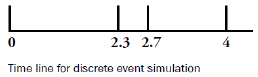
\includegraphics[width=150px]{img/DiskMod.png}
	\captionof{figure}{Abbildung einer diskreten Ereignis Modellierung}
	\label{fig:Abbildung einer diskreten Ereignis Modellierung}
\end{Figure}

      \subsubsection{Diskrete Raten Modellierung}
Charakteristika: Hybrid aus kontinuierlicher und ereignisorientierter Modellierung. Es werden Flüsse, die durch (bspw. Durchsatz-) Raten charakterisiert werden modelliert. Auf Grund von diskreten Ereignissen ändern sich die Raten.

      \subsubsection{Übersicht der Methoden}
Chapter03 - Ab Slide 25

   \subsection{Ablauf einer Simulationsstudie}
\textbf{1. Problembeschreibung}
\begin{itemize}
   \item Definition des genauen Problems, das untersucht werden soll
   \item Schriftliche Aussage über das Ziel der Problemstellung
\end{itemize}

\textbf{2. Modellierung des Systems und der Prozesse}
\begin{itemize}
   \item Was soll modelliert werden?
   \item Wie sind die Prozesse beschaffen?
\end{itemize}

\textbf{3. Datensammlung}
\begin{itemize}
   \item Welche realen Daten des Systems werden wie verwendet?
\end{itemize}

\textbf{4. Bau des Simulationsmodells}
\begin{itemize}
   \item Welche Prozesse sollen berücksichtigt werden?
   \item Wie werden diese modelliert?
   \item Welche Effekte werden vernachlässigt?
   \item Wie wird die Variablität beschrieben?
\end{itemize}

\textbf{5. Verfikation}
\begin{itemize}
   \item Macht das Modell, was es machen soll?
\end{itemize}

\textbf{6. Validierung}
\begin{itemize}
   \item Ist das Modell ein korrektes Abbild der Realität?
   \item Beschreibt das Modell die Wirklichkeit genügend gut?
\end{itemize}

\textbf{7. Durchführung von Experimenten}
\begin{itemize}
   \item Verschiedene Simulationsruns, um bestimmte Fragen zu beantworten
\end{itemize}

\textbf{8. Ergebnisanalyse und Interpretation}
\begin{itemize}
   \item Analyse der Ergebnisse (i.d.R. mit statistischen Auswertungen)
\end{itemize}

\textbf{9. Dokumentation}\\
\textbf{10. Umsetzung}

   \subsection{Algorithmus}
Der Simulationsalgorithmus
\begin{itemize}
   \item Eventliste L wird so geordnet, dass der EVent mit der kleinsten Ausführungszeit $t_k$ an erster Stelle steht. Dieser Event ist der Event, das als nächstes bearbeitet wird
   \item Die Bearbeitung dieses Events zur Systemzeit $t_{trigg}$ ($t_{trigg}$ Ausführungszeitpunkt des Events) $\rightarrow$ ändert den Systemzustand, $\rightarrow$ löst neue Events aus, $\rightarrow$ löscht pending Events
   \item Updaten der Even-List L $\rightarrow$ der erste Event (welcher gerade bearbeitet wurde) wird entfernt, $\rightarrow$ Eventliste neu sortieren, so dass der oberste Event dasjenige ist, das als nächstes ausgeführt wird.
\end{itemize}

\section{Markov Eigenschaften}

Dem Modell M/M/1 liegt die \textbf{Markov-Kette}.\\
Es handelt sich um einen Prozess mit abzählbar vielen Zuständen und gedächtnislosen Übergangswahrscheinlichkeiten.

\begin{Figure}
\centering
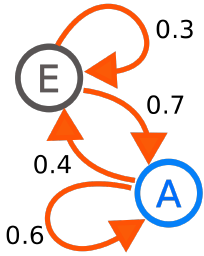
\includegraphics[width=150px]{img/MM1.png}
	\captionof{figure}{MM1 Modell}
	\label{fig:MM1 Modell}
\end{Figure}

   \subsection{Markov-Kette}
Die wichtigste Eigenschaft von Markov Ketten ist, dass ihr stochastisches Verhalten durch Übergangswahrscheinlichkeiten beschrieben werden kann.
\begin{equation}
   P[X(t_{k+1}) = x | X(t_k) = x']
\end{equation}
für Zustände X($t_k$) zum Zeitpunkt $t_k$ mit Zustandswerten x, x' und $t_k \leq t_{k+1}$\\
Wenn diese Übergangswahrscheinlichkeiten, sowie eine Häufigkeitsverteilung des Anfangzustandes gegebensind, ist es möglich, die Wahrscheinlichkeit jedes Zustands an jedem Zeitpunkt zu bestimmen.

      \subsubsection{Eigenschaft stoachastischer Prozesse}
$\rightarrow$ Eingangswahrscheinlichkeit aller Zustände X(0) = x zur Zeit $t_k = 0$ müssen in Summe 1 ergeben. 
\begin{equation}
   \sum P[x(T_k = 0) = x] = 1
\end{equation} 

$\rightarrow$ Alle von einem Zustand X(t_k) = x ausgehenden Übergangswahrscheinlichkeiten müssen 1 ergeben:
\begin{equation}
   \sum P[X(t_k+1) = x' | X(t_k) = x] = 1
\end{equation}

für Zustände X($t_k+1$) zum Zeitpunkt $t_k$

      \subsubsection{Regel für die Gesamtwahrscheinlichkeit}
In Markov-Ketten wollen wir die Gesamtwahrscheinlichkeit $p(x',x)$ für einen Übergang vom Zustand x in x' betrachten, unabhängig davon welches Ereignis diesen Zustandsübergang tatsächlich ausgelöst hat.\\
Wir wenden also die Regel für die Gesamtwahrscheinlichkeit an:
\begin{equation}
   p(x'|x) = \sum_i p(x' | x,i) * p(i|x)
\end{equation}

wobei p(i,x) die Wahrscheinlichkeit ist, dass Ereignis i im Zustand x eintritt; und p(x'|x,i) die Wahrscheinlichkeit, dass mit Ereignis i im Zustand x daraufhin Zustand x' eintritt.

      \subsubsection{Die Matrix der Übergangswahrscheinlichkeiten}
Die Informationen der Übergangswahrscheinlichkeiten in einer zeitdiskreten Markov-Kette wird in Matrixschreibweise adäquat beschrieben.\\
Wir definieren die \textit{transition probability matrix} \textbf{P}, welche aus den Koeffizienten $p_{ij}$ besteht:
\begin{equation}
   P \equiv [p_{ij}], i, j = 0,1,2,..,n
\end{equation}
wobei n die Anzahl Zustände im Zustandsraum angibt.\\

Dabei gilt: Alle Elemente jeder i-ten Zeile dieser Matrix, i=1,2,... müssen sich immer zu 1 addieren.
$$
\begin{bmatrix} 
p_{00} & p_{01} & .. & p_{0j} \\
p_{10} & p_{11} & .. & p_{1j} \\
p_{20} & p_{21} & .. & p_{2j} \\
\end{bmatrix}
$$

      \subsubsection{State transition Diagram}
\begin{Figure}
\centering
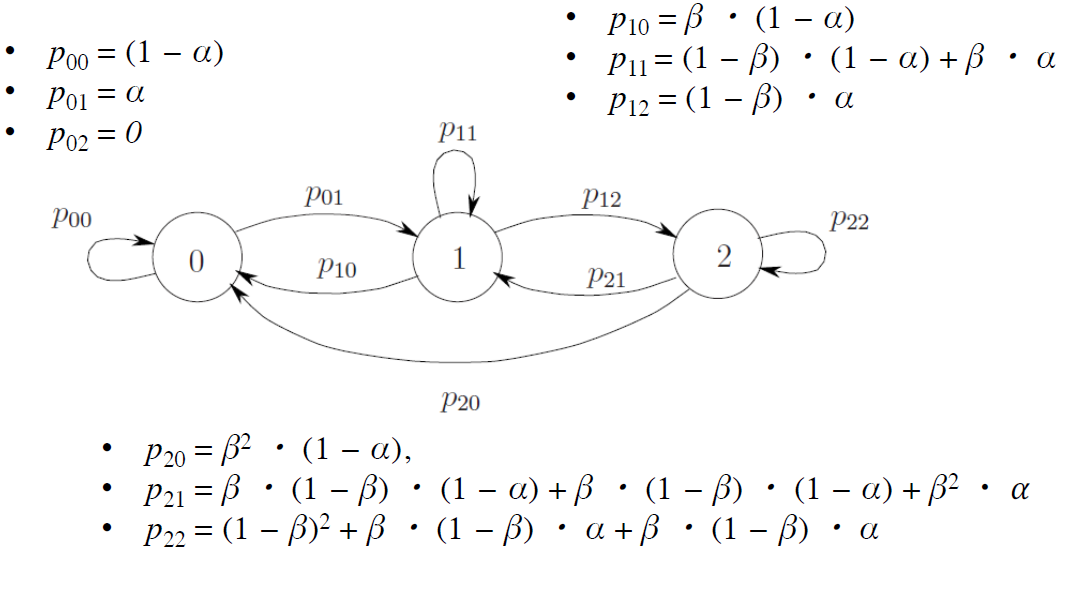
\includegraphics[width=150px]{img/STD.png}
	\captionof{figure}{Das State Transition Diagram}
	\label{fig:Das State Transition Diagram}
\end{Figure}

\section{Das Model M/M/1}
Die Kunden gelangen in die Schlange gemäss einem \textit{Poisson-Prozess}, d.h. die \textbf{Zwischenankunftszeiten} sind voneinander unabhängig, identisch \textbf{exponential-verteilte (iid)} Zufallsgrössen.\\
Die Dichte ist
\begin{equation}
   \listfunc f_A (t) = \lambda e^{-\lambda t}
\end{equation}

\begin{Figure}
\centering
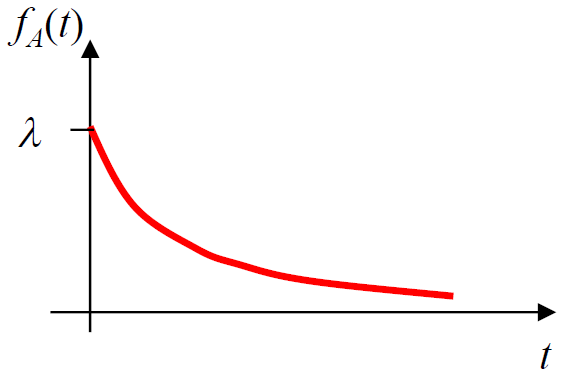
\includegraphics[width=150px]{img/MM1Graph.png}
	\captionof{figure}{Funktion MM1}
	\label{fig:Funktion MM1}
\end{Figure}
$\rightarrow$ $\lambda$ ist die mittlere Ankunftsrate \\
$\rightarrow$ $\frac{1}{\lambda}$ ist die mittlere Zwischenankunftszeit (d.h. der Erwartungswert der durch $f_A$ definierten Verteilung)\\

Eine \textbf{einzige} Bedienungsstelle kümmert sich um diese Kunden und zwar in der Reihenfolge FIFO. Die jeweiligen Bedienungszeit ist eine exponential-verteilte Zufallsgrösse mit Dichte:
\begin{equation}
   \listfunc f_s(t) = \mu e^{- \mu t}
\end{equation}

\begin{Figure}
\centering
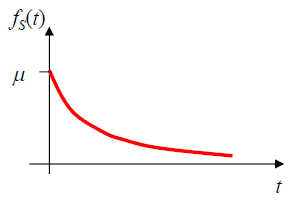
\includegraphics[width=150px]{img/midBedienungsrate.png}
	\captionof{figure}{Funktion mittlere Bedienungsrate}
	\label{fig:Funktion mittlere Bedienungsrate}
\end{Figure}
$\rightarrow$ $\mu$ ist die mittlere Bedienungsrate\\
$\rightarrow$ $\frac{1}{\mu}$ ist die mittlere Bediennugsdauer (d.h. der Erwartungswert $f_s$ definiertern Verteilung)

Die Anzahl $a(t)$ im Zeitintervall $[0,t)$ eingetroffener Kunden ist eine \textbf{Poisson-verteilte Zufallsgrösse} mit Erwartungswert $(\lambda t)$ es gilt 
\begin{equation}
   P[a(t) = k] = \frac{(\lambda t)^k}{k!} e ^{- \lambda t} : k = 0,1,2
\end{equation}

\begin{itemize}
   \item Ist das System im statistischen Gleichgewicht (stationär), so gilt dasselbe für die Anzahl Kunden b(t), die das System in diesem Zeitintervall verlassen.
   \item Im Folgenden wird die stationäre Verteilung der Anzahl $N(t)$ der zum Zeitpunkt $t$ im System anwesenden Kunden hergeleitet (für den Fall, dass t gegen unendlich strebt und das System stationär ist)
   \item Beruht das Warteschlangenverhalten auf dem Markoveigenschaften, dann lässt sich das System als \textit{single-server System mit unbegrenzter Kapazitätsauslastungsgrad und exponentialverteilten Interarrival- und Service-Zeitne} charakterisieren
   \item Es kann durch eine birth-death-Kette mit \textit{birth und death Parametern} Ankunftsrate: $\lamba_i = \lambda$ for all i = 0,1,... und Service-Rate $\mu_i = \mu$ for all i = 1,2,..
\end{itemize}
\begin{Figure}
\centering
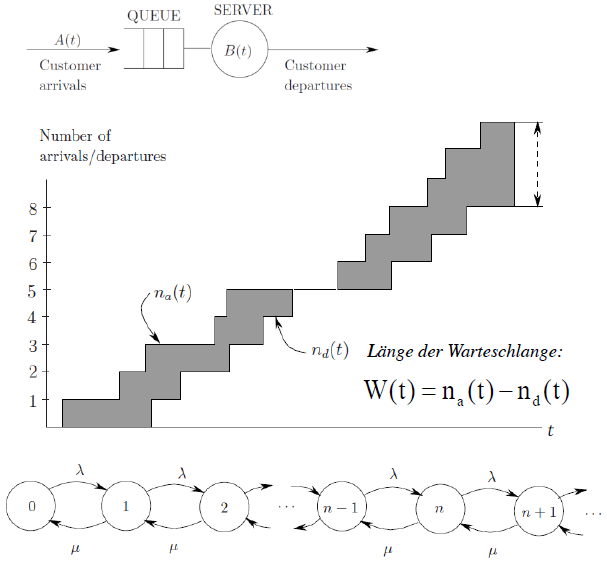
\includegraphics[width=150px]{img/stateTransitionRateDiagram.png}
	\captionof{figure}{Zustandsübergangsraten Diagramm}
	\label{fig:Zustandsübergangsraten Diagramm}
\end{Figure}

$\rightarrow$ Herleitung Chap03 ab Slide 56

      \subsubsection{Mittlere Anzahl Kunden im (stationären) System}
\begin{equation}
   \begin{split}

      E[N] &= \sum^\inf_{i=0} i \pi_i = \sum^\inf_{i=0} i(1-p) p^1 \\
      &= (1-p) \sum^\inf_{i=0} i p^i \\
      &= (1-p) p \sum^\inf_{i=0} i p^{i-1} \\
      &= \frac{p}{1-p}
      \rightarrow &= \frac{\lambda}{\mu-\lambda}

   \end{split}
\end{equation}
Wobei $\sum^\inf_{i=0} ip^{i-1} = \frac{1}{(1-p^2}$ die Ableitung von $\sum^\inf_{i=0} p^i = \fac{1}{1-p}$ ist

      \subsubsection{Mittlere Anzahl Kunden in der Schlange}
\begin{equation}
   \begin{split}

      E[N_q] &= \sum^\inf_{i=1} (i-1) \pi_i = \sum^\inf_{i=1} i \pi_i - \sum^\inf_{i=1} \pi_i = E[N]-(1-\pi_0) = \frac{p^2}{1-p} \\
      E[N_q] &= \frac{p^2}{1-p} = \frac{\lambda^2}{\mu(\mu - \lambda)}

   \end{split}
\end{equation}

   \subsection{Kennzahlen für Modell M/M/1}
\begin{Figure}
\centering
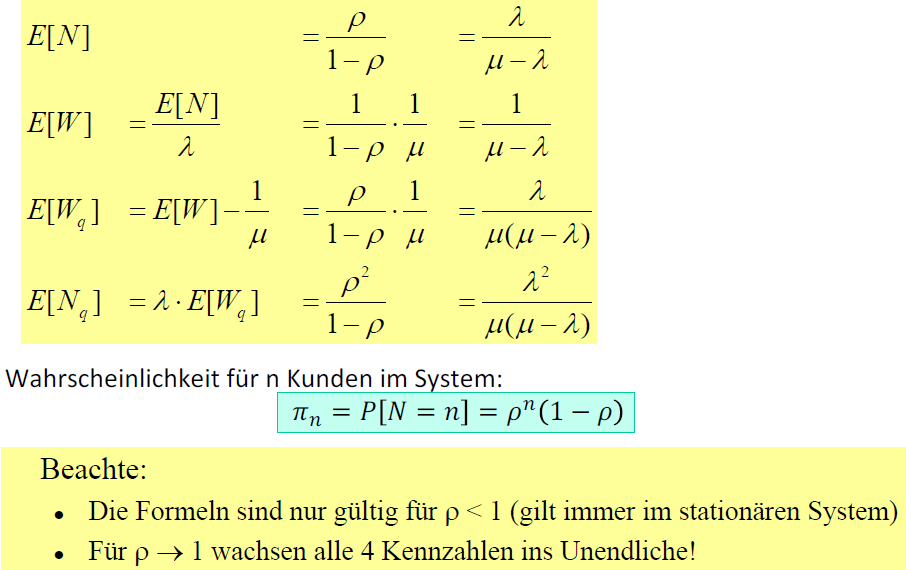
\includegraphics[width=150px]{img/KennzahlenMM1.png}
	\captionof{figure}{Überblick der Kennzahlen für das Modell MM1}
	\label{fig:Überblick der Kennzahlen für das Modell MM1}
\end{Figure}

\section{Das Model M/M/s}

\begin{itemize}
   \item Diese Schlange wird genauso wie das vorhergehende Modell M/M/1 analyisert
   \item Formel etwas kompliziert $\rightarrow$ Kein Problem, da Computer berechnet
   \item \textit{Geburts- und Sterbeprozess} liegt zu Grunde mit ähnlichem Übergangsgraphen
\end{itemize}

\begin{Figure}
\centering
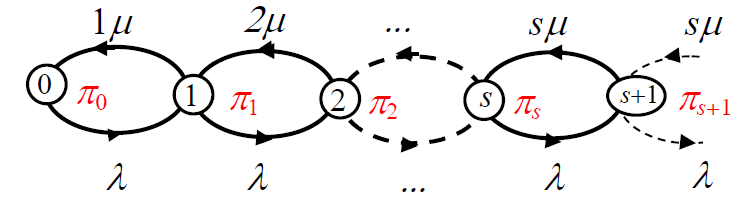
\includegraphics[width=150px]{img/UebergangsgraphenMMs.png}
	\captionof{figure}{Abbildung eines Überblickgraphen für das Modell MMs}
	\label{fig:Abbildung eines Überblickgraphen für das Modell MMs}
\end{Figure}

$\rightarrow$ Analog zum M/M/1-Fall, eine zugehörige Übergangsmatrix und ein Gleichungssystem zur Bestimmung der stationären Zustandswahrscheinlichkeiten $p_i$ i=0,1,2,... (Dies sei hier nicht explizit aufgeführt)

   \subsection{Lösung des Gleichungssystem}
\begin{Figure}
\centering
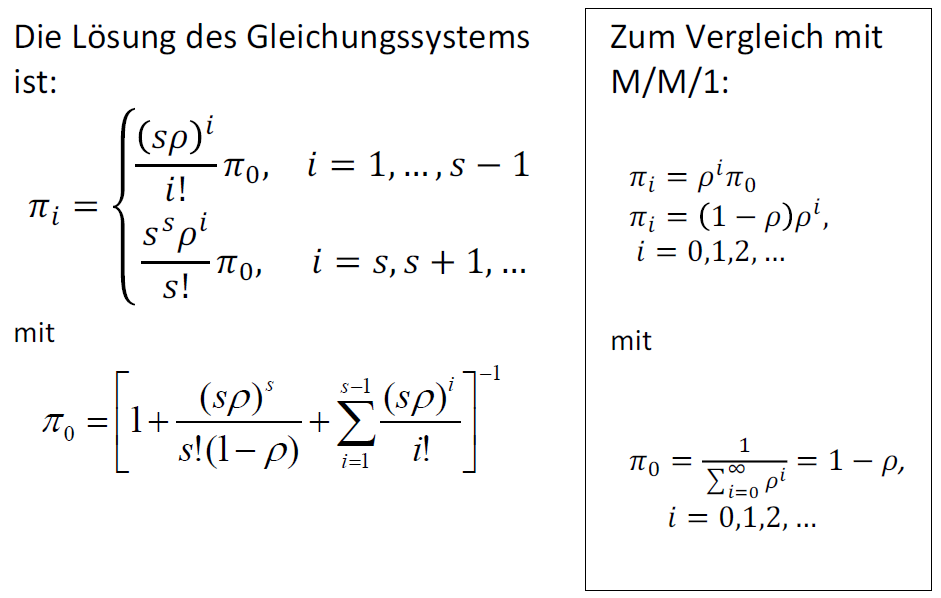
\includegraphics[width=150px]{img/LsgGLSMMs.png}
	\captionof{figure}{Lösung des Gleichungssystem für das Modell M/M/s}
	\label{fig:Abbildung eines Überblickgraphen für das Modell MMs}
\end{Figure}

\begin{Figure}
\centering
\includegraphics[width=150px]{img/BerechnungMMS.png}
	\captionof{figure}{Berechnungen für das Modell M/M/s}
	\label{fig:Berechnungen für das Modell MMs}
\end{Figure}

   \subsection{Verteilung der Wartezeit}
Für stationäre M/M/s Schlange ist es möglich, eine explizite Form der Verteilung $F(x)$ der Wartezeit $W_q$ abzuleiten:
\begin{Figure}
\centering
\includegraphics[width=150px]{img/VerteilungWartezeitMMS.png}
	\captionof{figure}{Verteilung der Wartezeit für das Modell M/M/s}
	\label{fig:Verteilung der Wartezeit für das Modell M/M/s}
\end{Figure}

\begin{Figure}
\centering
\includegraphics[width=150px]{img/VerteilungWartezeitMMSII.png}
	\captionof{figure}{Verteilung der Wartezeit (II)für das Modell M/M/s}
	\label{fig:Verteilung der Wartezeit (II) für das Modell M/M/s}
\end{Figure}

   \subsection{Kennzahlen für Modell M/M/s}
\begin{Figure}
\centering
\includegraphics[width=150px]{img/KennzahlenMMs.png}
	\captionof{figure}{Überblick der Kennzahlen für das Modell MMs}
	\label{fig:Überblick der Kennzahlen für das Modell MMs}
\end{Figure}


\chapter{Vorhersageverfahren}

\section{Vorhersagen im Operations Management}
$\rightarrow$ Auch Prognose oder Forecasting genannt\\
Dabei werden viele Entscheidungen des OM auf Vorhersagen getroffen:
\begin{itemize}
   \item Wirksamkeit und Nutzen von Entscheidungen abhängig von ungewisser Zukunft
   \item Verwendung von Vorhersagen zur Evaluation alternativer Entscheidungen
   \item Planung und Vorbereitung von betrieblichen Abläufen
\end{itemize}

   \subsection{Unterscheidung bezüglich Entscheidungsebene (Tragweite)}

\begin{itemize}
   \item Strategisch (langfristig, $\geq$ 2 Jahre) $\rightarrow$ bspw. Entwicklung neuer Produkte, Investitionen in Anlagen, Standortentscheide
   \item Taktisch (mittelfrisitg, Monate bis 2 Jahre) $\rightarrow$ bspw. Produktionsprogramm-Planung, Budgetplanung, Einkauf
   \item Operativ (kurzfristig, Tage bis Monate) $\rightarrow$ Lagerhaltung, Ablaufplanung
\end{itemize}

weitere Unterscheidungskriterien:
\begin{itemize}
   \item Ökonometrische Prognosen $\rightarrow$ Wirtschaftsindikatoren (Externe Quellen)
   \item Technologische Prognosen $\rightarrow$ Technologische Entwicklung bzgl Produkt, Analgen und Prozesse (interne und externe Quelle)
   \item Nachfrage-/ Bedarfsprognose $\rightarrow$ Bedarf von Endprodukte, Zwischenprodukte, Rohmaterialen, Analgenkapazität, Personal, Kapitel (interne und externe Quellen) $\rightarrow$ FOKUS
\end{itemize}

   \subsection{die 7 Schritte eines Forecasting}
Bspw. von DisneyChap 04 Slide 7\\

\begin{enumerate}
   \item Bestimmen der Verwendung der Vorhersage
   \item Auswahl der zu prognostizierenden Elemente 
   \item Auswahl des Prognosemodells
   \item Sammeln der erforderlichen Daten
   \item Prognose erstellen
   \item Ergebnis validieren und umsetzen
\end{enumerate}

   \subsection{Nachfrage- Bedarfsprognose}
Grundsätzlich unterscheidet man zwischen \textit{unabhängiger} und \textit{abhängiger} Bedarf\\

\textbf{unabhängiger Bedarf:} Bedarf an Endprodukten (bspw. Fahrräder)\\
\textbf{abhängiger Bedarf:} Bedarf der sich aus dem Bedarf von Endprodukten ergibt $\rightarrow$ Zwischenprodukte, Teilen, Rohmaterialen, Kapazität (bspw. Räder und Rahmen von Fahrräder)\\
$\Rightarrow$ Forecast bezieht sich auf \textbf{unabhängiger Bedarf} $\Rightarrow$ unabhängiger Bedarf kann teilweise beeinflusst werden (bspw. Preisaktionen)

   \subsection{Die drei Grundgesetze des Forecastings}
\textbf{1. Prognosen sind immer falsch}\\
\textbf{2. Detaillierte Prognosen sind schlechter als aggregierte Prognosen}
\begin{itemize}
   \item aggregierte Prognosen haben kleinere Variabilität als detaillierte
   \item $\rightarrow$ Prinzip des \textbf{Variability Pooling}
   \item bspw. Prognosen für Produktefamilien besser als für einzelne Produkte
\end{itemize}

\textbf{3. Je weiter Prognosen in die Zukunft reichen, desto weniger verlässlich sind sie}\\

      \subsection{Die Kunst der Prognosen}
\begin{itemize}
   \item Forecasting ist sowohl Wissenschaft als auch 'Kunst'
   \item Unterstützung durch breites Spektrum von quantitativen Modellen
   \item Entscheidungsfindung häufig in Zusammenspiel mit \textbf{qualitative} Informationen und Intuition von Fachleuten
   \item Beizug von Spezialisten oft empfehlenswert
\end{itemize}


\section{Prognoseverfahren: Eine Übersicht}

   \subsection{Qualitative Verfahren}

\begin{itemize}
   \item Häufig in langfristigen Prognosen
   \item Entwickeln von Zukunftsszenarien mit Hilfe von Wissen, Erfahrung und Intuition von Experten (bspw. Komitte von Verantwortlichen aus Marketing, Produktion, Finanzen)
   \item {\textbf{Delphi-Methode:} 
      \begin{itemize}
         \item Meist anonymisierte Befragung von Experten mittels Fragekatalog
         \item Oft iterativer Prozess: Mehrere Befragungsrunden, bis Antworten 'stabilisiert'
         \item Nach jeder Runde Aufarbeitung der Antworten und Entwurf eines neuen Fragekatalogs
         \item bspw. Voraussichtlicher Zeitpunkt der Einführung einer neuen Technologie
      \end{itemize}}
   \item Marktstudien, Kundenbefragung
   \item Analogieschlüsse (bspw. Nachfrage eines Produkts schätzen durch vergleichbare Produkte)
\end{itemize}

   \subsection{Quantitative Verfahren}

      \subsubsection{Zeitreihen-Modelle ('Time Series Models')}
\begin{itemize}
   \item Voraussage der zukünftigen Werten einer Variablen als eine Funktion von vergangenen Werten dieser Variablen $\rightarrow$ Prognose ausschliesslich gestützt auf einre Reihe vergangener Beobachtungen \textbf{Kein Erklärungsversuch} (bspw. Prognose der Nachfrage eines Produkts als Funktion der zurückliegenden Nachfrage)
   \item Diverse matehematische Modelle unterschliedlicher Komplexität: \textit{Glättungsverfahren, Box-Jenkins-Verfahren, Shiskin Time Series, Kalman Filter}
\end{itemize}

      \subsubsection{Kausale Modelle}
   \begin{itemize}
      \item Voraussage der zukünftigen Werte einer Variable ('interessierende Variable') als Funktion gewisser anderer Variablen ('ekrlärende Variablen') $\rightarrow$ Annahme einer kausalen Beziehung zwischen beiden Variablen \textbf{Erkärungsversuch} (bspw. Nachfrage eines Produkts in einer Region ('int. Variable') als Funktion vom Lohnniveau und Bevölkerungsdichte)
      \item Diverse mathematische Modelle: \textbf{Regressionsanalyse}
   \end{itemize}


\section{Komponenten einer Zeitreihe}
Eine Zeitreihe ist eine \textit{zeitliche Folge von beobachteten Werten ('Beobachtungen') einer gewissen Modellgrösse ('Variablen')}\\
Eine Zeitreihe X lässt sich in der Regel erklären durch die 'Überlagerung' von 4 Komponenten:
\begin{itemize}
   \item Trend \textbf{T} $\rightarrow$ bspw. Nachfrage-Zuwachs eines Produkts
   \item Zyklische Schwankungen \textbf{C} $\rightarrow$ bspw. Konjunkturzyklen
   \item Saisonale Schwankungen \textbf{S} $\rightarrow$ bspw. Nachfrageunterschiede Sommer/Winter
   \item zufällige Schwankungen \textbf{I} $\rightarrow$ Autokorrelation
\end{itemize}
Überlagerung im Sinne einer \textit{multiplikativen} oder \textit{additiven} Verknüpfung
\begin{itemize}
   \item \textbf{multiplikativ}: $X = T*C*S*I$
   \item \textbf{additiv}: $X = T+C+S+I$
\end{itemize}

\section{Zeitreihen-Modelle: Glättungsverfahren}
   \subsection{Bezeichnungen}
\begin{Figure}
\centering
\includegraphics[width=150px]{img/GlaettungsverfahrenBezeichnungen.png}
	\captionof{figure}{Überblick der Bezeichnungen eines Glättungsverfahren}
	\label{fig:Überblick der Bezeichnungen eines Glättungsverfahren}
\end{Figure}

* Als Beobachtungswert sei im Folgenden der Bedarf eines Produkts angenommen.

\begin{Figure}
\centering
\includegraphics[width=150px]{img/ZeitreihenModell.png}
	\captionof{figure}{Abbildung eines Zeitreihen-Modells}
	\label{fig:Abbildung eines Zeitreihen-Modells}
\end{Figure}

   \subsection{Glättungsverfahren bei gleichmässigem Bedarf}
Annahme: Bedarf unterliegt \textbf{nur zufälligen Schwankungen}, d.h. Zeitreihe hat nur Komponente I

      \subsubsection{Gleitender Durchschnitt ('Moving Average')}
\textbf{Parameter:}\\
$n$: Anzahl berücksichtigte Perioden, $n \geq 1$\\
$F(t)$: Durchschnitt der letzten $n$ Beobachtungen\\
   \textit{Smoothed Estimate}
\begin{equation}
      F(t) &= \frac{1}{n} \sum^t_{i=t-n+1} A(i)
\end{equation}

   \textit{Forecast}
\begin{equation}
   f(t+\rho) = F(t) \t \rho = 1,2,..
\end{equation}

Dabei ist $F(t+1) = F(t) + \frac{A(t+1)}{n} - \frac{A(t-n+1)}{n}$

      \subsubsection{Gewichteter, gleitender Durchschnitt ('Weighted Moving Average')}
\textbf{Parameter:}\\
$n$: Anzahl berücksichtigte Perioden, $n \geq 1$\\
$w_i$: Gewicht für Periode i, $i = 1,..,t$, wobei $w_i > 0$ und $\sum^t_{i=t-n+1} w_i=1$\\
$F(t)$: Gewichteter Durchschnitt der letzten $n$ Beobachtungen\\
Festlegen der Gewichte: Tendenziell den jüngeren Beobachtungen höhere Gewichte geben als den älteren\\
   \textit{Smoothed Estimate}\\
\begin{equation}
   F(t) = \sum_{i = t-n+1}^t w_i * A(i)
\end{equation}
   \textit{Forecast}
\begin{equation}
   f(t+\rho) = F(t) \t \rho = 1,2,..
\end{equation}

      \subsubsection{Exponentielle Glättung ('Exponential Smoothing')}
   Exponentielle Glättung ist einfach eine ausgefeilte \textbf{Gewichtete Moving-Average-Methode}, mit folgenden Merkregeln:

\begin{Figure}
\centering
\includegraphics[width=150px]{img/ExponentialSmoothing.png}
	\captionof{figure}{Merkregeln des Exponential Smoothing}
	\label{fig:Merkregeln des Exponential Smoothing}
\end{Figure}

\textbf{Effekte des Exponential Smoothing:}\\
\begin{Figure}
\centering
\includegraphics[width=150px]{img/EffektExponentialSmoothing.png}
	\captionof{figure}{Effekt des Exponential Smoothing}
	\label{fig:Effekt des Exponential Smoothing}
\end{Figure}

$\rightarrow$ Generelle Entwicklung Chap04 Slide 25

   \subsection{Glättungsverfahren bei einem Trend}
Annahme: Bedarf unterliegt \textbf{zufälligen Schwankungen} und einem \textbf{Trend} $\rightarrow$ Zeitreihe umfasst die \textbf{zwei Komponenten I und T}

      \subsubsection{Exponentielle Glättung mit (linearem) Trend}
\textbf{Paraemeter:}\\
$\alpha$: Glättungsparameter für Schätzwert, $0 \leq \alpha \leq 1$\\
$\beta$: Glättungsparameter für Trend, $0 \leq \beta \leq 1$\\
Falls $\alpha, \beta \rightarrow 0$: starke Glättung,\\
falls $\alpha, \beta \rightarrow 1$: schwache Glättung\\
   \textit{Smoothed Estimate}
\begin{equation}
   F(t) = \alpha * A(t) + (1-\alpha)*[F(t-1) + T(t-1)]
\end{equation} 

   \textit{Smoothed Trend}
\begin{equation}
   T(t) = \beta * [F(t) - F(t-1)] + (1-\beta) * T(t-1)
\end{equation}

   \textit{Forecast}
\begin{equation}
      f(t+\rho) = F(t)+\rho * T(t) \t \rho = 1,2,..
\end{equation}

\textbf{Aufbau}\\
\begin{Figure}
\centering
\includegraphics[width=150px]{img/Aufbau.png}
	\captionof{figure}{Aufbau der Exponentielle Glättung mit Trend}
	\label{fig:Aufbau der Exponentielle Glättung mit Trend}
\end{Figure}

\begin{Figure}
\centering
\includegraphics[width=150px]{img/Illustration.png}
	\captionof{figure}{Illustration der Berechnung der Exponentielle Glättung mit Trend}
	\label{fig:Illustration der Berechnung  Exponentielle Glättung mit Trend}
\end{Figure}

      \subsubsection{Glättungsverfahren bei Trend und Saisonalität}
D.h. Zeitreihe umfastt die zwei Komponenten I und T und S.\\
\textbf{Winters Methode}\\
\textit{Parameter:}\\
$\alpha$: Glättungsparameter für Schätzwert $0 \leq \alpha \leq 1$\\
$\beta$: Glättungsparameter für Trend $0 \leq \beta \leq 1$\\
$\gamma$: Glättungsparameter für Saisonalität $0 \leq \gamma \leq 1$\\
Falls $\alpha \beta \gamma \rightarrow 0$: Starke Glättung\\
Falls $\alpha \beta \gamma \rightarrow 1$: Schwache Glättung 
   \textit{Smoothed Estimate}
\begin{equation}
   F(t) = \alpha * \frac{A(t)}{c(t-N)} + (1-\alpha)*[F(t-1) + T(t-1)]
\end{equation}

   \textit{Smoothed Trend}
\begin{equation}
   T(t) = \beta * [F(t) - F(t-1)] + (1-\beta) * T(t-1)
\end{equation}

   \textit{Smoothed Saisonality}
\begin{equation}
   c(t) = \gamma * \frac{A(t)}{F(t)} + (1-\gamma) * c(t-N)
\end{equation}

   \textit{Forecast}
\begin{equation}
   f(t+\rho) = [F(t) + \rho * T(t)] * c(t+\rho - N), \t t+\rho = N + 1,..., 2N   
\end{equation}

   \textit{Initialisierung c(t) mit Saisonfaktor}
\begin{equation}
   c(t) = \frac{A(t)}{\sum^t_{i=t-N+1} \frac{A(t)}{N}}
\end{equation}


   \subsection{Beurteilung der Qualität von Prognosenverfahren}
Auflistung der häufig benutzen Masse zur Qualitätsbeurteilung.

   \textbf{Mittlere Absolute Abweichung (MAD, 'Mean Absolute Deviation')}\\
\begin{equation}
   MAD = \frac{ \sum^m_{i=1} \abs{ f(i) - A(i)} }{m}
\end{equation}

   \textbf{Mittlere Quadratische Abweichung (MSD, 'Mean Square Deviation')}\\
\begin{equation}
   MSD = \frac{ \sum^m_{i=1} [f(i)-A(i)]^2 }{m}
\end{equation}

   \textbf{Verzerrung ('BIAS')}
\begin{equation}
   BIAS = \frac{ \sum^m_{i=1} f(i) - A(i) }{m}
\end{equation}

      \subsubsection{Verwendung der Qualitätsmasse (in konkreter Anwendung)}
Unter Ausnützung von (möglichst umfangreichen) Vergangenheitsdaten:
\begin{itemize}
   \item Finden von geeigneten \textbf{Parametereinstellungen} ('Kalibrierung)
   \item \textbf{Vergleich} verschiedener \textbf{Prognoseverfahren}
\end{itemize}


\section{Kausale Modelle: Lineare Regression und Trendprojektion}

   \subsection{Einfache lineare Regression}
\begin{itemize}
   \item \textbf{Zweck}: Quantifizierung des funktionalen Zusammenhangs zwischen X (unabhängige Variable) und Y (abhängige Variable)
   \item \textbf{Hypothese}: Linearer Zusammenhang $Y = A + BX + $ Zufallsvariable mit E-Wert 0 $\rightarrow$ \textit{beachte}: Auch andere Beziehungen auf lin. Fall zurückführbar
   \item Beste Schätzungen für $\^{a}$ und $\^{b}$ von A und B anhang von Beobachtungen finden
   \item $X$: deterministische Variable mit Werten $x_1,...,x_n$ 
   \item $Y$: Zufallsvariable
   \item $\={x} := \frac{1}{n} \sum_{j=1}^n x_j$, $\={y} := \frac{1}{n} \sum^n_{j=1} y_j$
   \item Beste Schätzungen für $\^{a}$ und $\^{b}$: Wähle $\^{a}$ und $\^{b}$ so, dass $Q=\sum_{j=1}^n [y_j - E(Y_j)]^2$ minimal ist
\end{itemize}

\begin{Figure}
\centering
\includegraphics[width=150px]{img/linReg.png}
	\captionof{figure}{Berechnung für linReg}
	\label{fig:Berechnung für linReg}
\end{Figure}

   \subsection{Trendprojektion}
\begin{Figure}
\centering
\includegraphics[width=150px]{img/Trendprojektion.png}
	\captionof{figure}{Abbildung einer Trendprojektion}
	\label{fig:Abbildung einer Trendprojektion}
\end{Figure}

\begin{Figure}
\centering
\includegraphics[width=150px]{img/BspITrendprojektino.png}
	\captionof{figure}{Beispiel einer Trendprojektion}
	\label{fig:Beispiel einer Trendprojektion}
\end{Figure}

\begin{Figure}
\centering
\includegraphics[width=150px]{img/TrendprojektionMitSaisSchwaI.png}
	\captionof{figure}{Beispiel einer Trendprojektion mit saisonalen Schwankungen I}
	\label{fig:Beispiel einer Trendprojektion mit saisonalen Schwankungen I}
\end{Figure}

\begin{Figure}
\centering
\includegraphics[width=150px]{img/TrendprojektionMitSaisSchwaII.png}
	\captionof{figure}{Beispiel einer Trendprojektion mit saisonalen Schwankungen II}
	\label{fig:Beispiel einer Trendprojektion mit saisonalen Schwankungen II}
\end{Figure}

\begin{Figure}
\centering
\includegraphics[width=150px]{img/TrendprojektionMitSaisSchwaIII.png}
	\captionof{figure}{Beispiel einer Trendprojektion mit saisonalen Schwankungen III}
	\label{fig:Beispiel einer Trendprojektion mit saisonalen Schwankungen III}
\end{Figure}

   \subsection{Korrelationskoeffizienten für lineare Regressionen}
\begin{itemize}
   \item \textbf{Zweck:} Korrelationskoeffizienten geben die Stärke der linearen Abhängigkeit wieder
   \item Der Korrelationskoeffizienten $r$ ist ein Wert zwischen -1 (negative Werte: antikorreliert) und +1 (positive Werte: korreliert)
   \item Werte um 0 lassen vermuten, dass keine Korrelation vorliegt. Die Berechnung ist ähnlich wie die für die lineare Regression.
\end{itemize}

\begin{Figure}
\centering
\includegraphics[width=150px]{img/Korrelationskoeffizienten.png}
	\captionof{figure}{Korrelationskoeffizienten}
	\label{fig:Korrelationskoeffizienten}
\end{Figure}

      \subsubsection{Pearson'sche Korrelationskoeffizienten}
\textbf{obere Zeile}: Wiedergabe der Streuung der Punktewolke sowie die generelle Richtung der linearen ABhängig von x und y\\
\textbf{Mittlere Zeile}: Keine Information zur Steilheit. Verläuft die Punktewolke exakt waagerecht (mittleres Bild) kann aufgrund von $Var(Y) = 0$ gar kein Korrelationskoeffizienten berechnet werden\\
\textbf{Untere Zeile}: Schwachpunkt, nichtlineare Abhängigkeiten nur unzureichend erfasst\\


\textbf{Weitere Techniken}: $\rightarrow$ Chap04 Slide 62


\section{Monitoring und Steuerung von Forecasts}

   \subsection{Tracking Signal}
\begin{itemize}
   \item \textbf{Zweck}: Rollendes (nachgeführtes quantitatives Mass dafür, wie gut ein Forecast aktuelle Werte vorhersagt)
   \item \textbf{Berechnung}: Verhältnis der laufenden Summe der Forecast-Fehler (\textit{Running sum of the forecast errors [\textbf{RFSE}]}) zum mittleren absoluten Fehler (\textit{Mean absolute deviation [\textbf{MAD}]})
\end{itemize}

   \textbf{Tracking Signal}:
\begin{equation}
   \frac{RFSE}{MAD} = \frac{ \sum (A_i - f_i) }{ \frac{ \sum \abs{A_i - f_i} }{n} }      
\end{equation}

\begin{Figure}
\centering
\includegraphics[width=150px]{img/TrackingSignal.png}
	\captionof{figure}{Abbildung der Grafik zum Tracking Signal}
	\label{fig:Abbildung der Grafik zum Tracking Signal}
\end{Figure}


\chapter{Mathematische Optimierung}

%ToDo: 6.1 Fallstudie zusammenfassen

\section{Optimierungsmethoden}

   \subsection{Problemformulierung}
Ein allgemeines Optimierungsproblem (bzw. Optimierungsmodell) \prod kann wie folgt geschrieben werden:
   $\prod: max\{f(x): x \in S\}$, wobei $S \subseteq \mathbb{R}^n}$\\

\begin{itemize}
   \item Ein Problem heisst \textbf{eingeschränkt, falls S} $\subset \mathbb{R}^n$ $\rightarrow$ enthalten Restriktionen (Zulässigkeitsbedingungen), welche die Menge der \textbf{zulässigen Lösungen S} $\subseteq \mathbb{R}^n$
   auf eine echte Teilmenge von $\mathbb{R}^n$ beschränken $\Rightarrow$ Aufgabe eine geeignete funktionale Beschreibung der Restriktionen zu finden
   \item Ein Problem heisst \textbf{uneingeschränkt, falls} $S = \mathbb{R}^n$ 
   \item Allgemein lässt sich sage, dass eingeschränkte Probleme typischerweise schwieriger zu lösen sind als uneingeschränkte
\end{itemize}

   \subsection{Eingeschränkte Optimierungsprobleme}
\textbf{(i) Funktionale Restriktionen}:\\
Der Lösungsraum S wird durch
\begin{itemize}
   \item eine Anzahl $p \geq 0$ von Ungleichungen der Form $g_i(x) \leq 0$ und
   \item eine Anzahl $q \geq 0$ von Gleichungen der Form $h_j(x) = 0$ definiert: $S = \{ x \in G_1 \times G_2 \times ..	\times G_n : g_i(x) \leq 0, h_j(x) = 0}$ , i=1..p
\end{itemize}

\textbf{(ii) Nicht-funktionale Restriktionen}:\\
Der Lösungsraum S ist durhc gewisse 'nichtfunktionale' Restriktionen definiert, bspw. logische Prädikate, welche die zulässigen Elemente aufgrund bestimmter Eigenschaften aus einer Grundmenge auswählen:\\
\t $ S = \{x \in G_1 \times G_2 \times .. \times G_n: $ 'x hat gewisse Eigenschaften \} $\rightarrow$ bspw. $x \in \mathbb{Z}^n$: x ist eine Permutation der Zahlen 1,..,n

   \subsection{Maximierungs- und Minimierungsprobleme}
Optimierungsprobleme können Maximierungs- oder Mainimierungsprobleme sein. Es gilt:
\begin{equation}
   max \{f(x) : x \in S \} = - min \{-f(x): x \in S \}
\end{equation}
und $x^* \in S$ ist genau dann eine Optimallösung des Maximierungsproblems, wenn $x^*$ eine Optimallösung des Minimierungsproblems ist.
\begin{Figure}
\centering
\includegraphics[width=150px]{img/MinMax.png}
	\captionof{figure}{Abbildung der Min-Max-Optimierung}
	\label{fig:Abbildung der Min-Max-Optimierung}
\end{Figure}

   \subsection{Nachbarschaftsbegriffe}
Eine auf S definierte nachbarschaft ist eine (mengenwertige) Funktion der Form $N: S \rightarrow P(S)$ welche jedem Punkt $x \in S$ eine Menge von benachbarten Punkte N(x) zuordnet, wobei gelten soll, dass $x \in N(x)$.\\
$N(x)$ wird als die Nachbarschaft von x bezeichnet.

\begin{Figure}
\centering
\includegraphics[width=150px]{img/euklidischeNachbarschaft.png}
	\captionof{figure}{Abbildung der euklidische Nachbarschaft}
	\label{fig:Abbildung der euklidische Nachbarschaft}
\end{Figure}

   \subsection{globales und lokales Optimum}
Ein $x^* \in S$ ist (bzgl. Nachbarschaft) eine lokale Optimallösung und $f(x^*)$ ein lokales Optimum von $\prod$ falls $\eps > 0$ existiert, so dass $f(x^*) \geq f(x)$ für alle $x \in N_\eps (x^*) \cap S$
\begin{Figure}
\centering
\includegraphics[width=150px]{img/GlobLocOpt.png}
	\captionof{figure}{Funktion globales bzw lokales Optimum}
	\label{fig:Funktion globales bzw lokales Optimum}
\end{Figure}

   \subsection{Konvexe Menge}
\begin{Figure}
\centering
\includegraphics[width=150px]{img/KonvexeMenge.png}
	\captionof{figure}{Konvexe Menge}
	\label{fig:Konvexe Menge}
\end{Figure}

   \subsection{konvexe und konkave Funktion}
\begin{Figure}
\centering
\includegraphics[width=150px]{img/konvexKonkav.png}
	\captionof{figure}{konvexe vs konkave Funktion}
	\label{fig:konvexe vs konkave Funktion}
\end{Figure}

   \subsection{Konvex vs. nicht-konvex}
Konvexe Optimierung beschäftigt sich mit der Maximierung (bzw. Minimierung) einer konkaven (bzw. konvexen) Zielfunktion f über einem konvexen Lösungsraum S.\\
Sie spielen eine herausragende Rolle in der Optimierungstheorie, da sich die Suche nach einem globalen Optimum auf die Suche nach einem lokalen Optimum reduziert.

\begin{Figure}
\centering
\includegraphics[width=150px]{img/NichtKonvex.png}
	\captionof{figure}{Nicht konvex}
	\label{fig:Nicht konvex}
\end{Figure}

   \subsection{global vs. lokal}
Unter globaler Optimierung wird die Aufgabe verstanden, eine globale Optimallösung für ein Optimierungsproblem zu finden (oder festzustellen, dass keine solche existiert).\\
Bei lokaler Optimierung begnügt man sich mit dem Auffinden einer lokal optimalen Lösung. Trivialerweise ist das erstere mindestens so schwierig wie das zweite.
Viele Bereiche der Optimierungstheorie ausserhalb der konvexen Optimierung befassen sich hauptsächlich mit lokaler Optimierung, wie beispielsweise das Gebiet der allgemeinen nicht-linearen Optimierung.
\begin{Figure}
\centering
\includegraphics[width=150px]{img/globLoc.png}
	\captionof{figure}{global vs local}
	\label{fig:global vs local}
\end{Figure}

   \subsection{Kombinatorische Nachbarschaft}
Eine diskrete ('kombinatorische') Nachabrschaft in $\mathbb{Z}^n$ ist gegeben durch $N(x) = \{x' \in \mathbb{Z}^n: x'$

\begin{Figure}
\centering
\includegraphics[width=150px]{img/KombNachbarschaft.png}
	\captionof{figure}{Beispiel einer kombinatorische Nachbarschaft für $\mathbb{R}^2$}
	\label{fig:Beispiel einer kombinatorische Nachbarschaft für R2}
\end{Figure}

   \subsection{diskret vs. kontinuierlich}
\begin{Figure}
\centering
\includegraphics[width=150px]{img/DiskKont.png}
	\captionof{figure}{diskret vs kontinuierlich}
	\label{fig:diskret vs kontinuierlich}
\end{Figure}

   \subsection{linear vs. nichtlinear}
\begin{itemize}
   \item lineare Optimierung beschäftigt sich mit der Optimierung einer linearen Zielfunktin unter Berücksichtigung einer Anzahl linearer Restriktionen (Ungleichungen oder Gleichungen)
   \item Lineare Modelle liegen am Ursprung des Operations Research und weisen tief reichende mathematische Strukturen auf, welche es heutzutage erlauben, auch grosse Probleminstanzen effizient zu lösen
   \item Von zentraler Bedeutung für die Praxis sind Modelle der ganzzahligen Linearen Programmierung, bei welchen alle (oder einige) Entscheidungsvariablen auf ganzzahlige Werte beschränkt (also diskret) sind. 
\end{itemize}

   \subsection{Niveaumengen}
Niveaumengen spielen insbesondere bei der graphischen Darstellung von zwei- und dreidimensionalen Funktionen eine Rolle.
\begin{itemize}
   \item Sei $f: S \rightarrow \mathbb{R}$ mit $S \subseteq \mathbb{R}^n$. Die Niveaumenge $L_a$ von f zum Niveau $\alpha \in \mathbb{R}$ ist gegeben durch $L_\alpha (x) = \{ x \in S: f(x) = \alpha$
   \item Für eine n-dimensionale Funktion f sind die Niveaumengen von der 'Dimension' n-1 (oder kleiner)
   \item Im Fall n=2 sind die Niveaumengen typischerweise 'Linien' ($\rightarrow$ 1D) und werden auch Niveaulinien (geografisch: Höhenkurven) genannt
   \item Falls $f: \mathbb{R}^n \rightarrow \mathbb{R}$ eine lineare Funktion ist, d.h. $f(x) = c_1 x_1 + .. c_n x_n$ für ein $c \in \mathbb{R}^n$, entsprehcehn die Niveaumengen parallelen Geraden, wobei der Vektor $c$
   orthogonal zu diesen Geraden ist und das Niveau $\alpha$ zunimmt, wenn die Geraden in Richtung von a 'parallel verschoben' werden.
   \item Für n=2 sind sie typischerweise 'Flächen' (2D Mengen) und werden auch Niveauflächen genannt
\end{itemize}

\begin{Figure}
\centering
\includegraphics[width=150px]{img/Niveaumengen.png}
	\captionof{figure}{Abbildung von Niveaumengen}
	\label{fig:Abbildung von Niveaumengen}
\end{Figure}

\begin{Figure}
\centering
\includegraphics[width=150px]{img/NiveaumengenOrtho.png}
	\captionof{figure}{Abbildung von Niveaumengen II}
	\label{fig:Abbildung von Niveaumengen II}
\end{Figure}

   \subsection{Halbräume und Hyperebenen}
Sei $a \in \mathbb{R}^n$ und $b \in \mathbb{R}$. Die Mengen $H = \{x \in \mathbb{R}^n : ax \leq b \}$ wird ein \textbf{Halbraum} und die Menge $H' = \{ x \in \mathbb{R}^n: ax = b\}$ eine \textbf{Hyperebene} in $\mathbb{R}^n$
genannt. H' heisst die definierende Hyperebene von H. 
      \subsubsection{Hyperebene}
Für eine Hyperebene $H' = \{ x \in \mathbb{R}^n: ax = b\}$ wird der Vektor a als Normalenvektor bezeichnet.\\

$\rightarrow$ Es gilt: $a(x-x_0) = ax - ax_0 = b - b = 0$ für alle $x \in H'$, d.h. a ist orthogonal zu allen Parallelvektoren von H'

\begin{Figure}
\centering
\includegraphics[width=150px]{img/Hyperebene.png}
	\captionof{figure}{Abbildung einer Hyperebene}
	\label{fig:Abbildung einer Hyperebene}
\end{Figure}

   \subsection{Polyeder und Polytop}
      \subsubsection{Polyeder}
Ein \textbf{Polyeder P} in $\mathbb{R}^n$ ist der Durchschnitt einer endlichen Anzahl von Halbräumen in $\mathbb{R}^n$ d.h. $P = \{ x \in \mathbb{R}^n: Ax \leq b\}$ für ein $A \in \mathbb{R}^{m \times n}$
und $b \in \mathbb{R}^m$. Die Mengen $\{ x \in \mathbb{R}^n: a^i x = b_i$, heissen die definierenden Hyperebenen von P. \\
$\Rightarrow$ Ein Polyeder ist also die Lösungsmenge eines linearen Ungleichungssystems.


      \subsubsection{Polytop}
Ein \textbf{Polytop} in $\mathbb{R}^n$ ist ein begrenztes Polyeder, d.h. ein Polyeder $P = \{ x \in \mathbb{R}^n: Ax \leq b \}$ für welches $l, u \in \mathbb{R}^n$ existieren, so dass
$P = \{ x \in \mathbb{R}^n: Ax \leq b $, \t $l \leq x \leq u \}$

\begin{Figure}
\centering
\includegraphics[width=150px]{img/Polytop.png}
	\captionof{figure}{Beispiel eines Polytops in $\mathbb{R}^2$}
	\label{fig:Beispiel eines Polytops}
\end{Figure}

   \subsection{Geometrische Lösung von Linearen Programme in $\mathbb{R}^2$ und $\mathbb{R}^3$}

\begin{Figure}
\centering
\includegraphics[width=150px]{img/GeoLsgLinProg.png}
	\captionof{figure}{Geometrische Lösung von Linearen Programme}
	\label{fig:Geometrische Lösung von Linearen Programme}
\end{Figure}

   \subsection{Simplex-Algorithmus}
\textbf{Input:} Eine instanz eines Linearen Programms $\prod$:\\
$max \{cx: x \in \mathbb{R}^n\}$ mit $P = \{ x \in \mathbb{R}^n: Ax \leq b \} A \in \mathbb{R}^{m \times n}$ und rank(A) = n. Dazu eine zulässige Basisauswahl $B \subseteq \{1, ..,m\}$, $\abs{B} = n$\\

\textbf{Output:}\\
 Eine optimale Eckpunktlösung $v \in P$, falls $\prod$ beschränkt ist. Andernfalls eine 'Richtung' $d \in \mathbb{R}^n$, entlang welcher die Zielfunktion unbeschränkt wachsen kann.

\begin{Figure}
\centering
\includegraphics[width=150px]{img/BspSimplexAlgorithmus.png}
	\captionof{figure}{Beispiel zum Simplex-Algorithmus I}
	\label{fig:Beispiel zum Simplex-Algorithmus I}
\end{Figure}

\begin{Figure}
\centering
\includegraphics[width=150px]{img/BspSimplexAlgorithmusII.png}
	\captionof{figure}{Beispiel zum Simplex-Algorithmus II}
	\label{fig:Beispiel zum Simplex-Algorithmus II}
\end{Figure}

   \subsection{ganzzahlig-lineare Programmierung (engl. Integer Linear Program)}

\textbf{(i) LP:} Der Lösungsraum eines Linearen Programms entspricht einem Polyeder, und ein LP kann allgemein geschrieben werden als: $LP: max\{cx: x \in P\}$ mit $P = \{ x \in \mathbb{R}^n: Ax \leq b \}$\\
\textbf{(ii) ILP:} Ein ganzzahlig-lineares Programm hat somit als Lösungsraum die ganzzahligen Vektoren eines Polyeder und kann geschrieben wreden als: $ILP: max\{cx: x \in P \cap \mathbb{Z}^n \} $ mit $P = \{ x \in \mathbb{R}^n: Ax \leq b \}$
\begin{Figure}
\centering
\includegraphics[width=150px]{img/ILP.png}
	\captionof{figure}{ILP}
	\label{fig:ILP}
\end{Figure}

Die meinung, dass eine nahezu optimale Lösung für ein ILP einfach gefunden werden kann, indem das entsprechende LP (ohne Ganzzahligskeitsforderung) gelöst wird und die gefundene Optimallösung auf- bzw. abgerundet wird, ist weit verbreitet\\
Dabei kann die Optimallösung des ILP beliebig weit von der Optimallösung des LP 'entfernt' liegen.
$\Rightarrow$ Bei dieser Überlegung wird übersehen, dass durch Runden eventuell gar keine zulässige Lösung des ILP konstruiert werden kann.\\
\begin{Figure}
\centering
\includegraphics[width=150px]{img/ILPII.png}
	\captionof{figure}{ILP II}
	\label{fig:ILP II}
\end{Figure}


\section{CMPL}
<Coliop|Coin> Mathematical Programming Language ist eine mathematische Programmiersprache und ein System für mathematische Programmierung und Optimierungen für lineare Optimierungsprobleme.

\end{document}